\documentclass[]{article}
\usepackage[utf8]{inputenc}
\usepackage[T1]{fontenc}
\usepackage[autostyle=true]{csquotes}
\usepackage{amsmath}
\usepackage{graphicx}


\usepackage{tikz}
\usepackage{longtable}
\usepackage{float}
\usepackage{subcaption}
\usepackage{geometry}

\author{Ravshanbek Khodzhimatov} 
\title{Welfare Effects of Individualizing Life-Cycle Pension Investments\\to Households in Turkey}

\begin{document}

\maketitle

\begin{abstract}
\vspace{20pt}
We review the current state of Turkish pension system and the history and developments of financial economics. We apply Munk's (2016) individualized lifecycle investment model to simulate Turkish retirement process, and compare the welfare effects with default retirement portfolio options provided by retirement funds or suggested by classical portfolio theory. We find that for upper-to-middle class citizens, individualizing portfolios in Munk's sense results in considerable welfare increases. 
\end{abstract}


\section{Introduction} % Main chapter title
\label{intro} % For referencing the chapter elsewhere, use \ref{introduction} 


\subsection{Theory and heuristics of life-cycle investments}
One of the most important investment decisions individuals face in their lives is investment in retirement portfolio. Since the birth of concept of retirement over a century ago, the various advisors have been ubiquitous. They tried to consult people on best ways to invest their money to afford a good standard of living during their old ages. The field of financial economics, however, started analyzing this type of investment decades later, starting from Markowitz's Modern Portfolio Theory (1952). Therefore, this field of theoretical economics has been heavily intertwined with empirical findings of non-academic financial consultants.
\paragraph*{}
In time, financial economists found inefficiencies in portfolio allocations suggested by finacial advisors (Campbell \& Viceira, 2002) and came up with quantitative solutions that would increase investors' welfare. The rapid adoption of Defined Contribution (DC) pension plans, where individuals choose their own pension investment funds and amounts freely, has made it even easier to adopt portfolio decisions described in formulas by economists. At the same time this shifted the whole responsibility on the individuals, and this opened a room for confusion among non-experts, who then decided to naively allocate 50\% of their money to risky assets and the other 50\% to riskless assets.
\paragraph*{} 
To address this issue, lifecycle investment strategies have been introduced by some institutions. They constituted the predefined percentages of risky and riskless fund investments for all ages until retirement. Such portfolios would be in compliance with theory that younger people should invest more in risky assets because this would increase expected earnings and in case of fault, they will be able to reallocate before getting older, and older people should invest more conservatively in less risky assets because they won't have enough time to recover from potential losses. Such "investment menus" were designed to help laymen make their decisions easier while still complying with complex theory. Alas, Turkish consulting firms have not included easy-to-comprehend lifecycle strategies (investment menus) in their bulletins and didn't try to spread transparent information. We will fill this important gap in our paper, but firstly we will recap the state of Turkish pension system.

\subsection{Turkish pension system}
The main pension funds in Turkey have been public for a long time: three main options existed: SSK for public and private sector workers, ES for civil servants, and Bag-Kur for self-employed workers and farmers. In 2006 they all merged into SGK. Private pensions have gained pace recently. As of January, 2017 a new clause of Turkish Labor Law came into action, that automatically enrolled every wage earner younger than 45 years into "Individual Retirement Scheme" --- a private pension fund. To further incentivize people not to opt out, the government promised to subsidize 25\% of their monthly contributions (as long as this wouldn't exceed 25\% of minimal wage). According to PwC research, this has tremendously increased fund sizes. Under the current system individuals may retire after contributing to a pension fund for at least 10 years and at least reaching the age of 56.
\paragraph*{}
The largest retirement funds in Turkey are listed in the table 1. All of them offer 3-4 default investment options with varying degrees of riskiness but they are not lifecycle investment strategies mentioned above. They also provide flexible investment options with ability to change portfolio allocation up to six times a year, but they are not very popular as they assume active involvement in their own portfolio and require a certain level of financial literacy. Not much academic research has been done on Turkish pension systems, and the existing research doesn't provide easy solutions. A recent example of this is Iscanoglu-Cekic's (2016) paper which doesn't consider life cycles and uses dynamic programming in the solution, which is also not accessible to wide audience.

\begin{table}
	\centering
	\caption{Largest Turkish Pension Funds}
	\begin{tabular}[H]{lc}
		\hline
		Fund name&Fund size\\
		\hline
		Anadolu Hayat Emeklilik&8.7 bln\\
		Garanti Emeklilik ve Hayat&7.4 bln\\
		AvivaSA Emeklilik ve Hayat&9.1 bln\\
		Allianz Yasam ve Emeklilik&6.8 bln\\
		Vakif Emeklili&3.5 bln\\
		\hline
	\end{tabular}\\
	Source: Pension Monitoring Center (2016)
\end{table}

\subsection{Focus of this paper}
In this paper we will consider the general framework of lifecycle investments and its historical evolution within the field of financial economics. We will take a look at standard heuristics suggested by financial consultancies and compare their welfare outcomes with those of optimal solutions given by theory. We will use the latest theoretical findings by Munk (2016) and show that optimal solutions can be both efficient and easy to comprehend without use of complex dynamic optimization results.
\paragraph*{}Next chapter will review all the relevant literature in this field and show the theoretical developments. Chapter 3 will summarize the theoretical framework and model we will use in our simulation. Chapter 4 will explain the data sources and the structure of our simulation. Chapter 5 will present the results of the simulation and Chapter 6 will conclude our findings. The used sources will be listed in References chapter. All the relevant proofs will be available in Appendices. 




\section{Literature Review}
\label{litreview}

\subsection{Beginnings of financial economics}

The financial economics is generally thought to be started with Modern Portfolio Theory (MPT) by Markowitz (1952). He pioneered the mean-variance analysis and was followed by Mutual Funds Separation Theorem of Tobin (1958). The premise of the model was, that if investors care only about the return and the volatility (modelled by mean and variance (or standard deviation) respectively) over a single period, then there is a straight line representing a fixed ratio of risky assets in the optimal portfolio. We summarize their model below.

\subsubsection{Mean-variance analysis}
Let there be two assets, risky and risk-free with returns $R$ and $R_f$ respectively. Let $\alpha$ be the ratio of total wealth invested in a risky asset. Then the portfolio return is:

\begin{center}
  $R_p = \alpha E[R] + \left(1-\alpha \right) R_f$
\end{center}

\paragraph{}We want to choose $\alpha$ that maximizes the expected return and minimizes the volatility of the portfolio. Markowitz solves the following unconstrained optimization problem:

\begin{center}
  $\displaystyle\max_{\alpha} \{ E[R_p] - \frac{\gamma}{2}\sigma^2_p \}$
\end{center}

where $\gamma$ is risk-aversion coefficient. The classical solution is:

\begin{center}
	$\alpha = \frac{E[R] - R_f}{\gamma\sigma^2}$
\end{center}

\paragraph{}This is a crucial result used a lot in industry, academia and MBA courses but most importantly, revived recently by Munk (2016) which we will explore later in this chapter. The issue with this basic model was that it demanded fixed risky asset ratio for everybody and thus could not explain (i) why younger investors take more risks than older ones and (ii) why aggressive investors invest more in stocks than bonds compared to the conservative ones. The model also didn't include loss aversion of people, because although this solution performs best on average in the long run, when it underperforms, it does so in a high way and investors are willing to sacrifice possible gains for loss avoidance.

\paragraph{}Following Markowitz, Merton (1970) and Samuelson (1969) introduced a framework to understand long term portfolio investments using changes in investment opportunities during the life. Their result was to repeat the Markowitz's myopic choice in every period. Formally he stated that whenever the relative risk aversion does not depend on wealth, the time horizon is not important for an investor. The Merton solution was not adopted outside academia because it failed to justify the financial rules of thumb like "young should invest more aggresively" and because it used a dynamic programming approach without general closed form solution, which finance analysts found complicated (Campbell and Viceira 2000).



\subsection{Advancements in thought}

\paragraph*{}Merton (1971) added labor into the model and found that when the markets are complete and labor income is constant and risk-free, the optimal portfolio choice is:

\begin{center}
	$\alpha_t = \frac{\mu - R_f}{\gamma \sigma^2}(\frac{W_t + H_t}{W_t})$
\end{center}

Which meant that adding labor income into the model increased the risky asset ratio in the portfolio choice. The idea of considering labor income was further advanced with the collaboration of Merton and Samuelson with Zvi Bodie in their paper Bodie et al. (1992) where they introduced a notion of human capital to the problem. They formalized the view that labor income is a divident on individual's lifelong human wealth. It is non-tradeable because of moral hazard problem (any future claims of immediate salary for the promise of working for years to come are not enforcable as they constitute some form of slavery). Introducing human capital came as follows: they let individuals solve two problems simultaneously each period --- (a) the decision between consumption and leisure and (b) the decision of allocating portfolio between risky and riskless assets. The framework is that individuals maximize their lifetime utility from consumption and leisure:

\begin{center}
	$E_t \left[\displaystyle\int_0^T e^{-\delta s} u(C(s), L(s))ds \right]$
\end{center}

The risky asset and labor income both follow the Ito's process:

\begin{center}
	$\frac{dP}{P} = E_t[R]dt + \sigma dz$,\\
	$\frac{dw}{w} = E_t[ROR_w]dt + \sigma^* dz^*$
\end{center}

For convenience, only special cases of $\sigma^* \in \{0, k\sigma \}$ are considered. Bodie et al. summarized their method in a very accessible way. The timing is in 5 steps:

\begin{enumerate}
	\item At the beginning of time $t$, the individual calculates the present value of his future earnings and finds its risk characteristics. This value is called a human capital at time $t$ and is denoted by $H(t)$.
	\item The total wealth at time $t$ is defined as a sum of human wealth and financial wealth: $W(t) = F(t) + H(t)$.
	\item The individual determines the optimal wealth allocated to consumption of a numeraire good and leisure.
	\item The individual solves for $\hat{x}(t)$ --- the percentage of total wealth $W(t)$ invested in a risky asset.
	\item Subtract the wage's implicit exposure to risk from Step 1 from the total amount to be invested in a risky asset $\hat{x}(t) \cdot W(t)$.
\end{enumerate}

\paragraph*{}The result was that since the optimal risky investment ratio was calculated from the total wealth, the outside observer trained using classical theory, who only sees the financial wealth and not the human wealth, could not explain why it is rational to invest such a large portion of a financial wealth in a risky asset. According to this model, though, the ratio invested in risky asset was not very high, because it considered the total wealth. This also meant that when people get older, their human capital, which is calculated as a present value of the future labor income streams, gradually depletes. Therefore, as an investor gets older, $H(t)$ approaches $0$, the total wealth $W(t)$ approaches the financial wealth $F(t)$, which means that older people are advised to invest a smaller percentage of their financial wealth into risky assets than younger people. The paper claimed that this result holds under so-called "normal circumstances" but empirics did not confirm that view because many young people didn't invest in risky assets at all. 

\paragraph*{}Cocco et al. (2005) solved the same problem numerically and simulated the investment processes using calibrated and conventional parameters. They introduced the heterogeneity in the model and considered different educational levels, marital status and family sizes of investors. Their results were complementary to Bodie et al. in a sense that they studied incomplete markets. These results were complex but a referee of this paper suggested the following simplification (which was then incorporated in the paper):

\begin{center}
	$\alpha_t = \begin{cases} 100\% & t<40\\(200-2.5t)\% & t\in[40,60]\\50\% & t>60 \end{cases}$,
\end{center}

where $\alpha_t$ is the investment share in risky assets and $t$ is investor's age.

\paragraph*{}Flavin and Yamashita (2002) used mean-variance analysis to study how including housing as a separate investment instrument will affect life-cycle investment behavior. They simplified the above model by excluding human capital and risk-free asset from the model. Nevertheless, the results were substantial. They found that due to the large magnitude of housing investment (which is both investment and consumption good) in utility function, when consumers are forced to satisfy particular housing constraint, it exceeds their risk capacity and they tend to not invest in risky assets at all. This explained why young people don't invest in stocks empirically. They also found that introducing housing added individualization into model: similar households would invest different amounts depending on their housing wealth. Ascheberg et al. (2013) found the long-term cointegration among housing, stocks and labor income. They found similar results explaining young people's non-participation in stock markets. 



\subsection{Reinvention of analytical solution}


\paragraph*{}Munk (2016) showed how simple one-period mean-variance analysis can be expanded to capture all the life-cycle effects mentioned above without any need for dynamic programming and numerical solutions. His model resembled Bodie et al. (1992) but did not use numerical approach. Munk considered a decision between single risk-free asset with return $r_f$ and a vector of risky assets (including housing investment) with return $r \sim (\mu, \Sigma)$. The control variable was $\pi$ --- a vector of shares of total wealth invested in each of risky assets with return $r$. Munk transformed Markowitz's optimization problem to capture dynamics:


\begin{center}
	$ \displaystyle\max_{\pi} \{ E[\frac{W_1}{W_0}] - \frac{\gamma}{2} var(\frac{W_1}{W_0}) \} $
\end{center}

where total wealth is a sum of financial and human wealth: $W_t = F_t + L_t$ and human capital has returns $r_L \sim (\mu_L, \sigma_L)$. Munk derived the following solution (which can be obtained from calculus):

\begin{center}
	$\pi^* = \frac{1}{\gamma} \frac{W_0}{F_0} \cdot \Sigma^{-1} (\mu - r_f \cdot 1) - \frac{L_0}{F_0} \cdot \Sigma^{-1} cov(r,r_L)$
\end{center}

The solution captured all the results of the previous papers and was a lot more intuitive. So, for example, if human capital is very correlated with stocks, then the risky asset investment $\pi^*_{risky}$ is crowded out. Or, when a person gets old, her human capital depletes and the second term goes to zero and the solution replicates the Merton solution.

\paragraph{}It is worth noting that Munk added housing as purely financial investment and not a tool for heterogeneity as other papers below tried to do. 

\subsection{Relevant research}
Olear (2016) used Munk (2016) to study the welfare gains of individualized life-cycle retirement investments as opposed to standardized ones. She used Ascheberg's human capital, stocks and labor income correlation structure and Cocco et al. (2005)'s labor income process to model the standardized life-cycles and Munk's solution to model the individualized profiles. Unlike Munk, she added housing capital as a pre-existing wealth with mortgage loan independent of other financial investments. She found positive welfare gains when individualized investments were used for retirement on the data for Netherlands.




\section{Model}
\label{model}

\subsection{Labor income process}

We model the labor income process as a function of individiual characteristics plus aggregate and idiosyncratic shocks for working people, and as the percentage $\lambda$ of the last received wage for the retired. This is summarized in Cocco et al. (2005) as follows:

\begin{center}
	$\log(Y_{it}) =
		\begin{cases}
			f(t,Z_{it}) + v_{it} + \epsilon_{it}, & t \leq T \\
			log(\lambda) + f(T, Z_{iT}) + v_{iT}, & t > T
		\end{cases}
	$
\end{center}

where $T$ is the retirement age and $f(t, Z_{it})$ is the log-wage regression outcome for individual $i$ at time $t$. The error terms are decomposed as:

\begin{center}
	$v_{it} = v_{i,t-1} + u_{it}$,\\
	$u_{it} = \xi_t + \omega_{it}$
\end{center}

and distributed as:

\begin{center}
	$u_{i} \sim N(0, \sigma^2_u)$,\\
	$\xi \sim N(0,\sigma^2_{\xi})$,\\
	$\omega_{i} \sim N(0, \sigma^2_{\omega})$.
\end{center}

We use Olear's (2016) approach (Appendix B) to transform the main equation into the following:

\begin{center}
	$Y_{i,t+1} = 
	\begin{cases}
		Y_{it} (1 + g_{i,t+1} + \xi_t + \omega_{it}), & t \leq T \\
		\lambda (1 + f(T, Z_{iT}) + v_{iT}), & t > T
	\end{cases}	
	$
\end{center}

where $g_{i,t+1} = f(t+1, Z_{i,t+1}) - f(t, Z_{it})$, $\xi$ is the aggregate shock and $\omega_{i}$ is idiosyncratic shock.


\subsubsection{Correlations}

To derive the above equation, we must construct the aggregate labor income shock $\xi$. Following the Approach of Ascheberg et al. (2013) we want labor income series to be correlated with both stock series and housing series. To do that we first create three uncorrelated standard normally distributed random series $\epsilon_{st}$, $\epsilon_{ht}$, $\epsilon_{yt}$ and multiply them by the Cholesky decomposition $Q$ of the correlation matrix $R$, i.e. $R = QQ'$, where:

\begin{center}
	$R = \begin{bmatrix}
					1 & \rho_{sh} & \rho_{sy} \\
					\rho_{hs} & 1 & \rho_{hy} \\
					\rho_{ys} & \rho_{yh} & 1
			\end{bmatrix}
	$
\end{center}

Stock, housing and labor income series then take the form of expected rate of return plus the volatility multiplied by the modified error terms. For details please refer to Appendix A:\\
$\frac{\Delta S_{t+1}}{S_t} = \mu_s + \sigma_s \cdot \epsilon_{st}$\\
$\frac{\Delta H_{t+1}}{H_t} = \mu_h + \sigma_h \cdot \left(\rho_{hs}\epsilon_{st} + (\sqrt{1-\rho^2_{hs}})\epsilon_{ht}\right)$\\
$\frac{\Delta Y_{t+1}}{Y_t} = \mu_v + \sigma_v \cdot \left(\rho_{ys}\epsilon_{st} + \left(\frac{\rho_{yh} - \rho_{sh}\rho_{sy}}{\sqrt{1-\rho^2_{sh}}}\right)\epsilon_{ht} + \left(\sqrt{1-\rho^2_{ys}-(\frac{\rho_{yh} - \rho_{sh}\rho_{sy}}{\sqrt{1-\rho^2_{sh}}})^2}\right)\epsilon_{vt}\right)$


\subsubsection{Calibration}

To do our simulation, we must calibrate the above model parameters from the historical labor income data. The calibration is done using data obtained from the repeated cross-sectional study by TUIK (2003-2014). Aggregating these studies results in a pseudo-panel, which we will use to summarize labor income dynamics.

\paragraph{}
In summarizing the series we will use simple medians and means. In determining the expected values of time-series parameters, we will use simple arithmetic mean and standard deviation.

\paragraph{}
In constructing the simulated labor income series, we used kinked ordinary least-squares (OLS) estimations with kinks at ages of 35 and 45 separately for every education level $i$:

\begin{center}
	$\Delta\log (wage_{it}) = \alpha_0 + \alpha_1 \cdot d_{35} + \alpha_2 \cdot d_{45} + \alpha_3 \cdot t$
\end{center}




\subsection{Welfare measurement}
Similarly to Cocco et al. (2005) we use CRRA utility function in our model:

\begin{center}
	$E_1[U(c)] = E_1 \left[\displaystyle\sum^T_{t=1} \delta^{t-1} \displaystyle\prod^{t-1}_{j=0} p_j \cdot \frac{c^{1-\gamma}_{it}}{1-\gamma}\right]$
\end{center}

where $p_k$ is the probability of survival from time $k-1$ to time $k$. Note that we omitted the bequest motives from the original formulation, thus retired person consumes all of his income at any given time.

%\paragraph*{}Following Olear (2016) we use certainty equivalent consumptions (CEC) instead of expected utilities to compare the welfare effects between different lifecycle choices. Appendix C shows the calculation of the following formula for CEC:

%\begin{center}
%	$CEC = \left( \frac{E[U(c)]\cdot(1-\gamma)}{\sum^T_{t=1} \delta^{t-1} \prod^{t-1}_{j=0} p_j} \right)^{1/(1-\gamma)}$
%\end{center}


\subsection{Individualization}

To derive the individual lifecycle portfolios for every wealth type we use a special case of Munk (2016) with housing investment and human capital included. The similar approach and its solution has been done by Olear (2016), but she included housing capital as a pre-existing wealth bought for an outside mortgage, independent of the investment decision. In this paper, we consider housing as a purely financial investment, in line with Munk (2016). Munk provides the following optimal asset allocation:


\begin{center}
	$\pi_{t+1} = \frac{\mu_s - r_f}{\gamma \sigma^2_s}  + \frac{L_t}{F_t} \cdot \left(\frac{\mu_s - r_f}{\gamma \sigma^2_s} - \frac{\rho_{SL}\sigma_L}{\sigma_S} \right)$
\end{center}

without housing investment, and:

\begin{center}
	$\pi_{t+1} = \frac{1}{\gamma (1 - \rho^2_{SH}) \sigma_S} \cdot \frac{W_t}{F_t} \left( \frac{\mu_s - r_f}{\sigma_S} - \rho_{SH} \frac{\mu_h - r_f}{\sigma_h} \right) - \frac{L_t}{F_t} \cdot \frac{\sigma_L}{\sigma_S} \frac{\rho_{SL} - \rho_{SH}\rho_{HL}}{1 - \rho^2_{SH}}$\\
	$\pi_{h,t+1} = \frac{1}{\gamma (1 - \rho^2_{SH}) \sigma_H} \cdot \frac{W_t}{F_t} \left( \frac{\mu_h - r_f}{\sigma_h} - \rho_{SH} \frac{\mu_s - r_f}{\sigma_s} \right) - \frac{L_t}{F_t} \cdot \frac{\sigma_L}{\sigma_h} \frac{\rho_{HL} - \rho_{SH}\rho_{SL}}{1 - \rho^2_{SH}}$
\end{center}

when housing is considered as a second risky financial investment. In line with Munk (2016), we calculate the risk free asset share as $\left( 1 - \pi - \pi_h \right)$ and only then impose constraints. If any of the above shares is negative, we equate it to zero, and if the sum of remaining shares exceeds $1$, we divde all of the shares by their sum to obtain a proportionate asset allocation. 

\subsection{Retirement income}

The funds invested in retirement are modeled to be paid back in annuities. Thus, we ignore the case when some share of matured fund can be withdrawn immediately. Further, in order for our individualization analysis (based on house posessions) to have an effect, we also use reverse mortgages proposed. In theory, reverse mortgages pay retired individuals fixed annuity in return for inheriting the house after she dies. This is a plausible tool, because we ignore all bequest motives, and it liquidifies the housing posessions, although it is not yet available for Turkish investors. 

\paragraph{}So, at the age of 57, the price of owned house is calculated and is added to the matured pension amount ($MP$) to obtain total wealth:

\begin{center}
	$W_{57} = H_{57} + MP$
\end{center}

All of the $W_{57}$ is used to buy an annuity which will repay an individual $\frac{W_{57}}{1+\sum^{100}_{t=58} \frac{p_t}{1+r_f}}$ annually. The calculation details are available in Appendix D. 



\subsection{Data Structure and Sources}
\label{data}

In our simulation we will compare welfare effects of default lifecycles and individualized lifecycles defined below. The magnitutes and sources of parameters are given in the next section. Default lifecycles are taken from the ones mentioned in our Literature Review chapter and from the real investment strategies of the largest Turkish pension fund provider Anadolu Hayat Emeklilik. Individualized lifecycles will be calculated using Munk's optimal portfolio formula from previous chapter taking idiosyncracies into consideration.

\subsection{Data}

To measure the stock series we used BIST 30 index which measures the aggregate performance of 30 best companies in Turkey. The monthly data is taken from Borsa Istanbul. We can see from Figure 1 the general upward trend with collapse during 2008 crisis.

\begin{figure}
	\centering
    \begin{minipage}{0.45\textwidth}
		\centering
		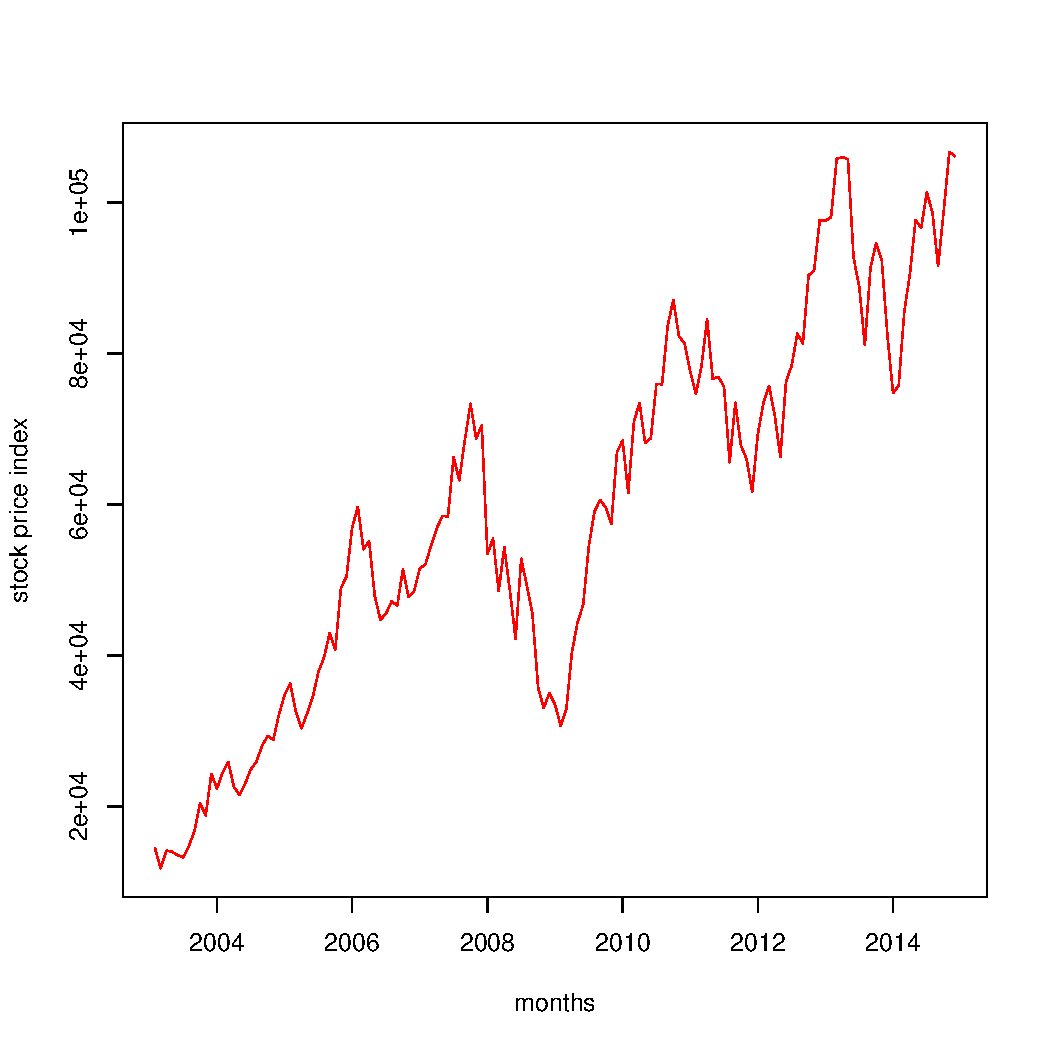
\includegraphics[scale=0.4]{figs/bist.pdf}
		\caption{BIST30 Turkish stock market performance index}
	\end{minipage}
	\hfill
    \begin{minipage}{0.45\textwidth}
		\centering
		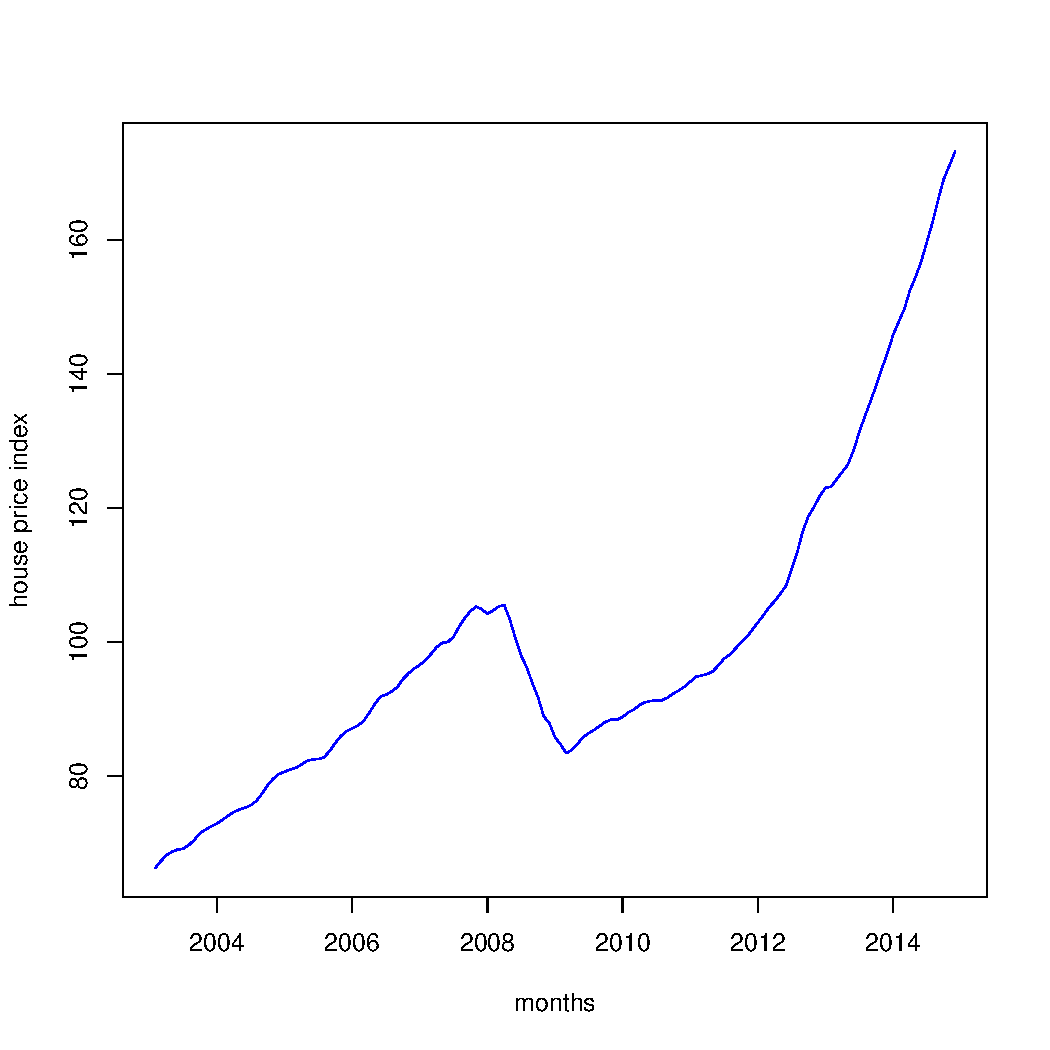
\includegraphics[scale=0.4]{figs/reidin.pdf}
		\caption{Reidin Turkish house price index}
	\end{minipage}
\end{figure}

\paragraph{}We used Reidin AEINDEXF index to obtain data on house prices in Istanbul. The historical dynamics of this index are illustrated in Figure 2.

\paragraph{}We used TUIK's Household Budget Survey Data and regression results of Aktug, Kuzubas, Torul (2017). We have 55 thousand panel data points for 170 households for 2001 to 2014 years. We can observe the hump-shaped lifetime income distribution in Figure 3. This corresponds well to an established literature in this field.

\begin{figure}[h]
	\centering
	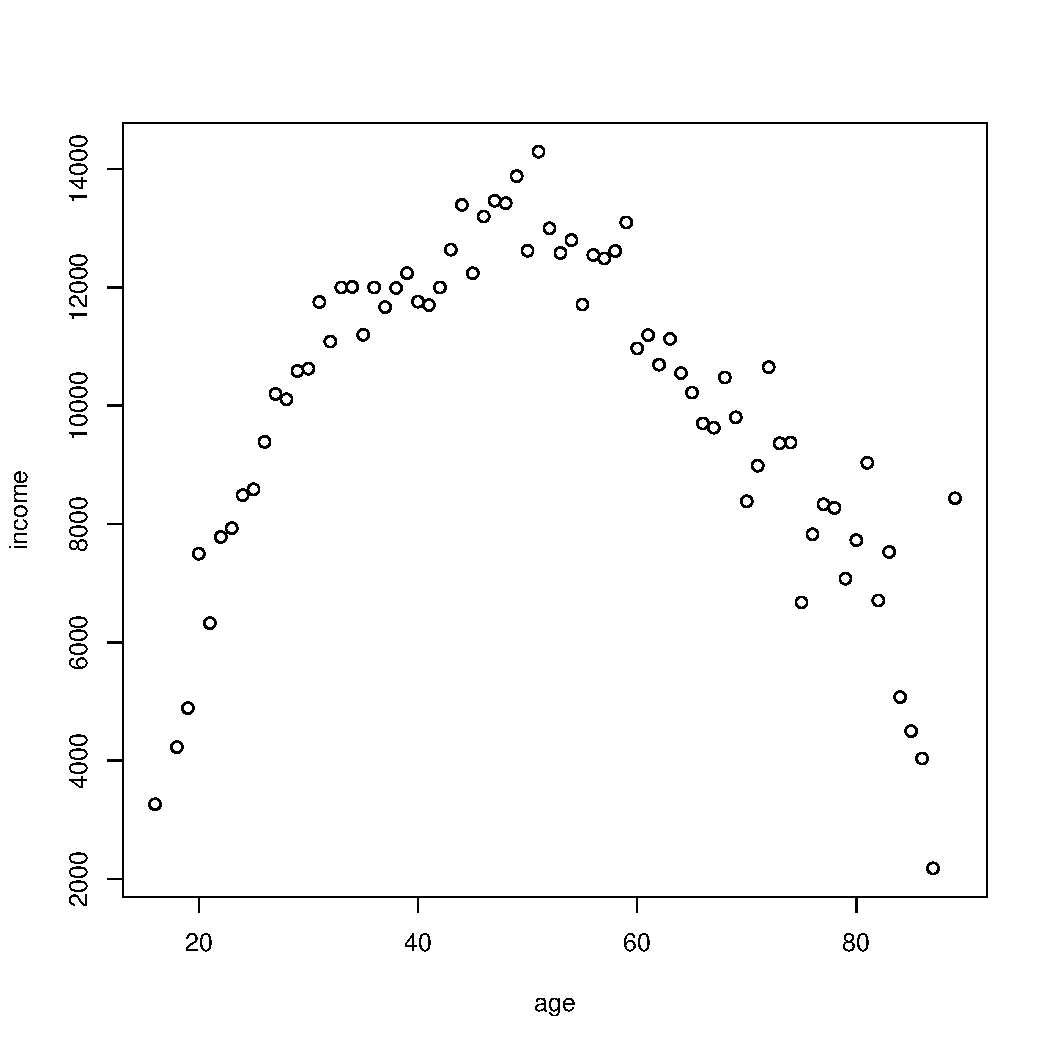
\includegraphics[scale=0.6]{figs/wage2median.pdf}
	\caption{Median Turkish salaries by age}
\end{figure}

\subsubsection{Default parameters}
In our simulation we start with a 28 years old individual who invests in her retirement for 30 years until she reaches retirement at 57. We set the default coefficient of relative risk aversion at $5$, but, in line with Torul et al. (2018), we check the sensitivity for $1.5$ and other values. Also, according to Torul et al. (2018), we set the subjective discount rate at $0.89$.

\paragraph{}Stock returns for Turkey were estimated from historical data to be equal to $23.2\%$ annually, with standard deviation $36\%$. Risk-free rate forecasts are obtained from OECD Data Bank (2018) and are equal to $10.8\%$ per annum.

\paragraph{}Housing capital appreciation averaged at $8.3\%$ with $9.5\%$ standard deviation. But in our simulation we have excluded the temporary housing price drop during 2008 crisis to clear from macroeconomic effects. Therefore, in our simulation, housing capital appreciaton averaged at $11.3\%$ with $5.2\%$ standard deviation.

\paragraph{}Aggregate wage growth series showed $5.5\%$ standard deviation.

\paragraph{}The correlations between house and stock prices, and house prices and wages gave $0.24$ and $0.37$ respectively.

\paragraph{}The data on survival probability for all ages has been taken from Turkish Statistical Institute's (TUIK) database and illustrated in Figure 4. All of these findings have been summarized in Table 2. 

\begin{figure}[h]
	\centering
	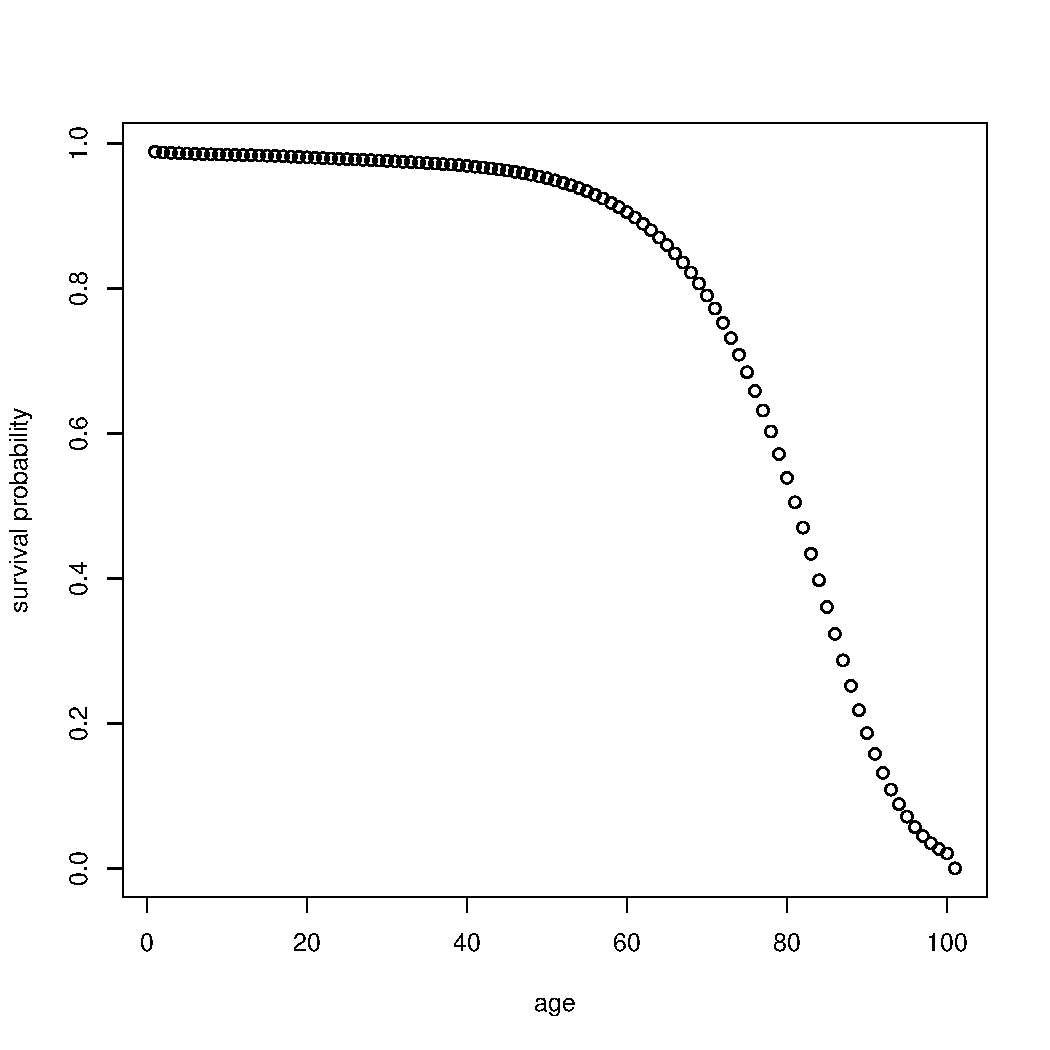
\includegraphics[scale=0.6]{figs/survival.pdf}
	\caption{Survival probabilities by age}
\end{figure}

\begin{table}
	\centering
	\caption{Benchmark Parameters}
	\begin{tabular}[c]{lll}
		\hline
		Parameter&Description&Value\\
		\hline
		$Y$&Beginning age&$28$\\
		$R$&Retirement age&$57$\\
		$T$&Lifespan (years)&$100$\\
		$\gamma$&Risk aversion&$5$\\
		$\beta$&Discount rate&$0.89$\\
		$r_f$&Risk-free rate&$0.108$\\
		$\pi$&Average inflation rate&$0.084$\\
		\hline
		$\mu_s$&Expected stock returns&$0.232$\\
		$\mu_h$&Expected housing returns&$0.113$\\
		$\sigma_s$&Stock returns volatility&$0.36$\\
		$\sigma_h$&Housing returns volatility&$0.052$\\
		$\sigma_w$&Wage growth volatility&$0.056$\\
		$\rho_{hs}$&Housing-stock correlation&$0.24$\\
		$\rho_{hw}$&Housing-wage correlation&$0.37$\\
		\hline
		$p_{28}$&Survival probability at age 28&$0.977$\\
		$p_{57}$&Survival probability at age 57&$0.924$\\
		$p_{100}$&Survival probability at age 100&$0$\\	
		\hline
	\end{tabular}
\end{table}


\subsubsection{Heterogeneity parameters}
In the same manner as Olear(2014) we will use wage growth rate, stock-income correlation and idiosyncratic labor income risk to model heterogeneities in education and sector. Let's now consider the heterogeneities one at a time:

\paragraph{Heterogeneity in education}
In line with Olear's (2016) approach we model the heterogeneity in education using the differences in wage growth rates. Indeed, we expect the salaries for higher education level to grow faster than for the lower education level. Some of this expectation comes from the fact that people with lower education are restricted in their career ladders and cannot rise very high in a workplace. Another intuition is that while college dropouts start working immediately, college graduates and graduate students continue to study and thus report zero income. When they graduate, their salary immediately rises from zero to the average salary, and this constitutes a steeper wage growth curve at the beginning of their lives. Figure 5 shows the wage series for different levels of education. Note that the curves for the lowest education levels are practically flat and the those for the highest education levels have varying non-zero slopes. 

\begin{figure}[h]
	\centering
	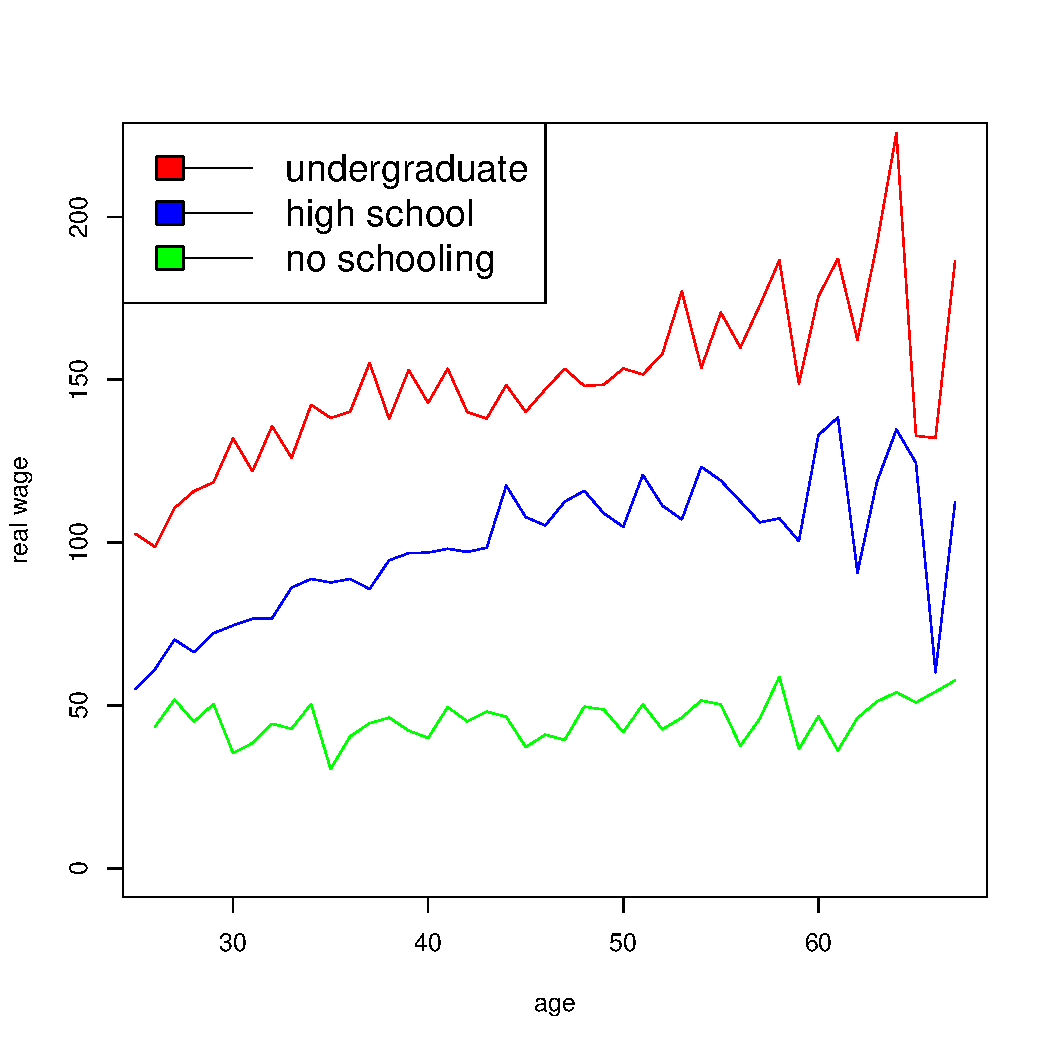
\includegraphics[scale=0.6]{figs/wage2educ.pdf}
	\caption{Lifetime wage dynamics by education level}
\end{figure}

Performing kinked regressions of log wages on ages, as described in the previous chapter, yielded best linear fits for three different education levels of our choice: postgraduate, high school, and no schooling. The corresponding labor income growth rates can be characterized as steep, moderate, and flat respectively. We considered wage data until 60 years, as Turkish retirement age is at 57, and have added empirically best kinks at ages 35 and 45. The results are summarized in Table 3 and illustrated in Figure 6. In this figure red lines represent the actual wages dynamics for postgraduate, high school, and no schooling, and blue lines are plots of the percentage changes proposed in Table 3, where the starting points all correspond to the actual starting points from the data. Figure 7 illustrates the same parameterized curves without actual wage curves. 

\begin{table}
	\centering
	\caption{Estimated Benchmark Wage Growth Rates $\mu_w$}
	\begin{tabular}[c]{l|ccc}
		Age&Flat&Moderate&Steep\\
		\hline
		0-35&0\%&3.5\%&6.5\%\\
		36-45&0\%&3\%&2\%\\
		46-60&0\%&0\%&0\%\\
	\end{tabular}
\end{table}


\begin{figure}[h]
	\centering
    \begin{minipage}{0.45\textwidth}
		\centering
		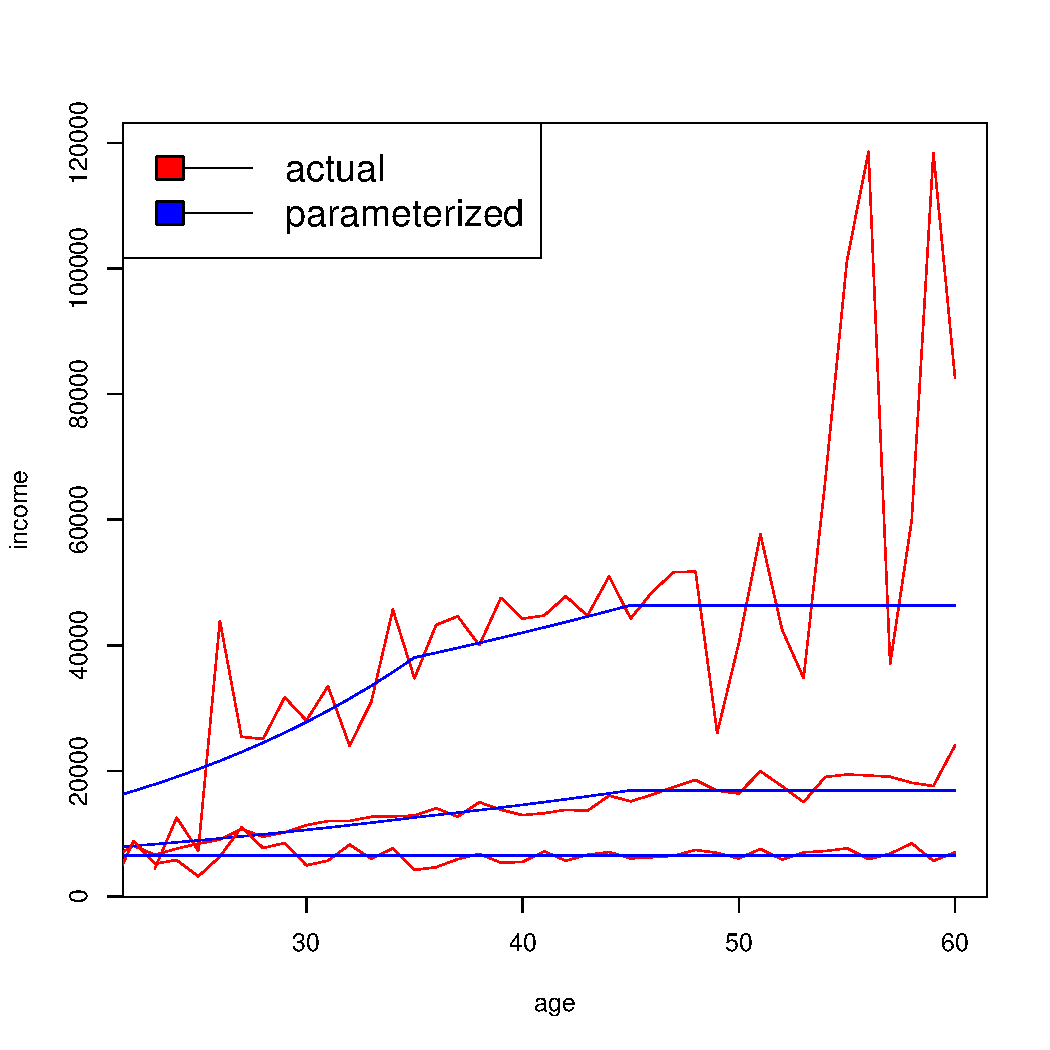
\includegraphics[scale=0.4]{figs/heterwage.pdf}
		\caption{Actual and parameterized benchmark wage dynamics by age}
	\end{minipage}
	\hfill
    \begin{minipage}{0.45\textwidth}
		\centering
		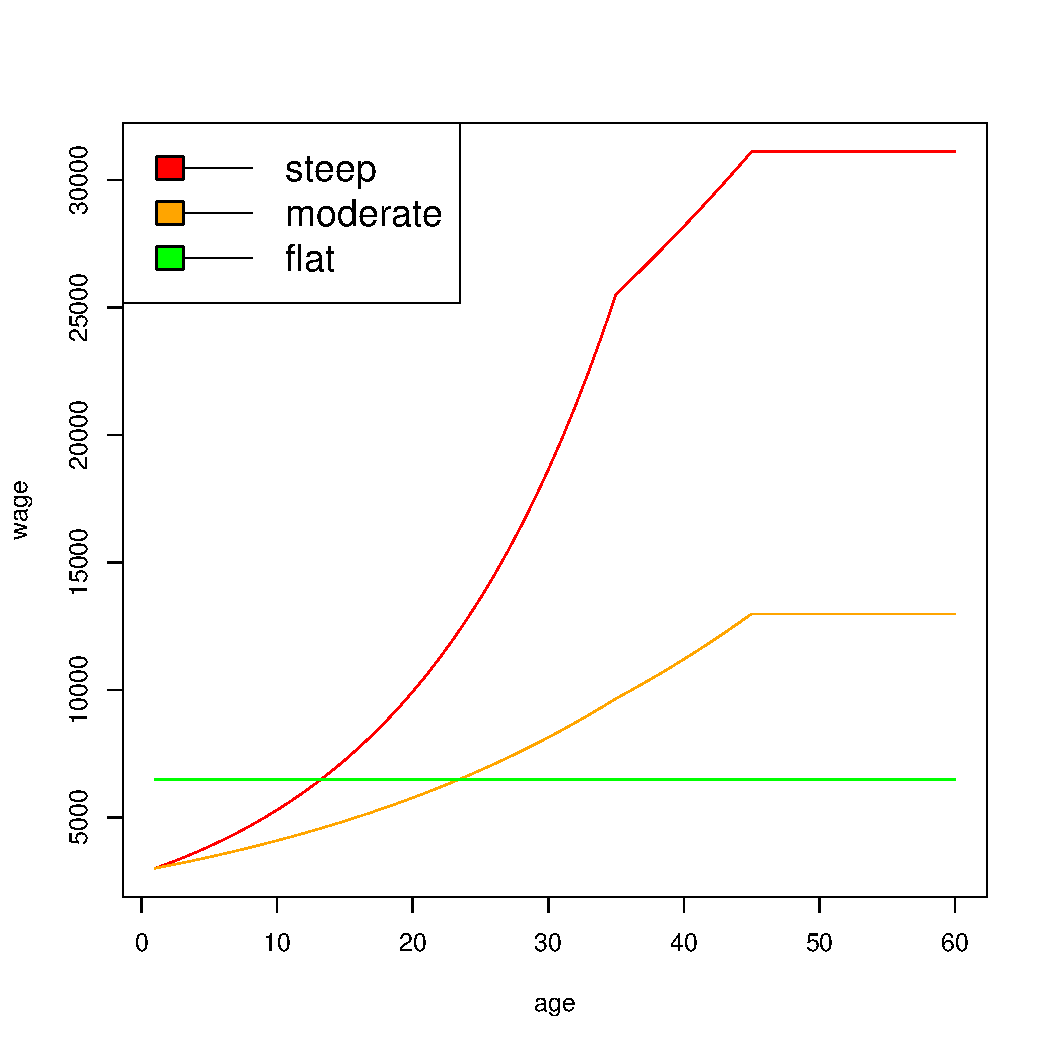
\includegraphics[scale=0.4]{figs/heterwageless.pdf}
		\caption{Parameterized wage dynamics by age}
	\end{minipage}

\end{figure}


\paragraph{Heterogeneity in sectors of work}

As we explained in Chapter 3, we model our labor income series as functions of age, gender, education, sector of work etc. We already showed in previous section how we incorporated the heterogeneity in education. We also stated at the beginning of this chapter that we consider only male individuals as heads of households; age is implicit in our analysis. In this section we will model the differences in sectors of work. Again, similar to Olear's (2016) approach we model these differences using correlations of wage growth rates with stock market returns. Indeed, it is expected that sectoral wages would be proportional to the stock returns only to the extent of their exposure to stock markets. In that sense, the stock-wage correlations are expected to be zero for public sector, where wages are fixed regardless the markets, and high in financial institutions. When we juxtaposed wages by sector and stock prices we obtained very high correlations, which was expected due to the economic growth over the years represented in Figure 8. Therefore we divided the wages by price levels to obtain the real wages, and, as expected, we obtained more realistic correlations. The financial sector's correlations were as high as $0.44$  and public sector, social service and education's were as low as $0.08$. Thus, our expectations that different sectors have different wage-stock correlation $\rho_{sw}$ were confirmed and we decided on three measures of $\rho_{sw}$ as our simulation benchmarks: $0$, $0.2$ and $0.4$ as stated in Table 4.

\begin{figure}[h]
	\centering
	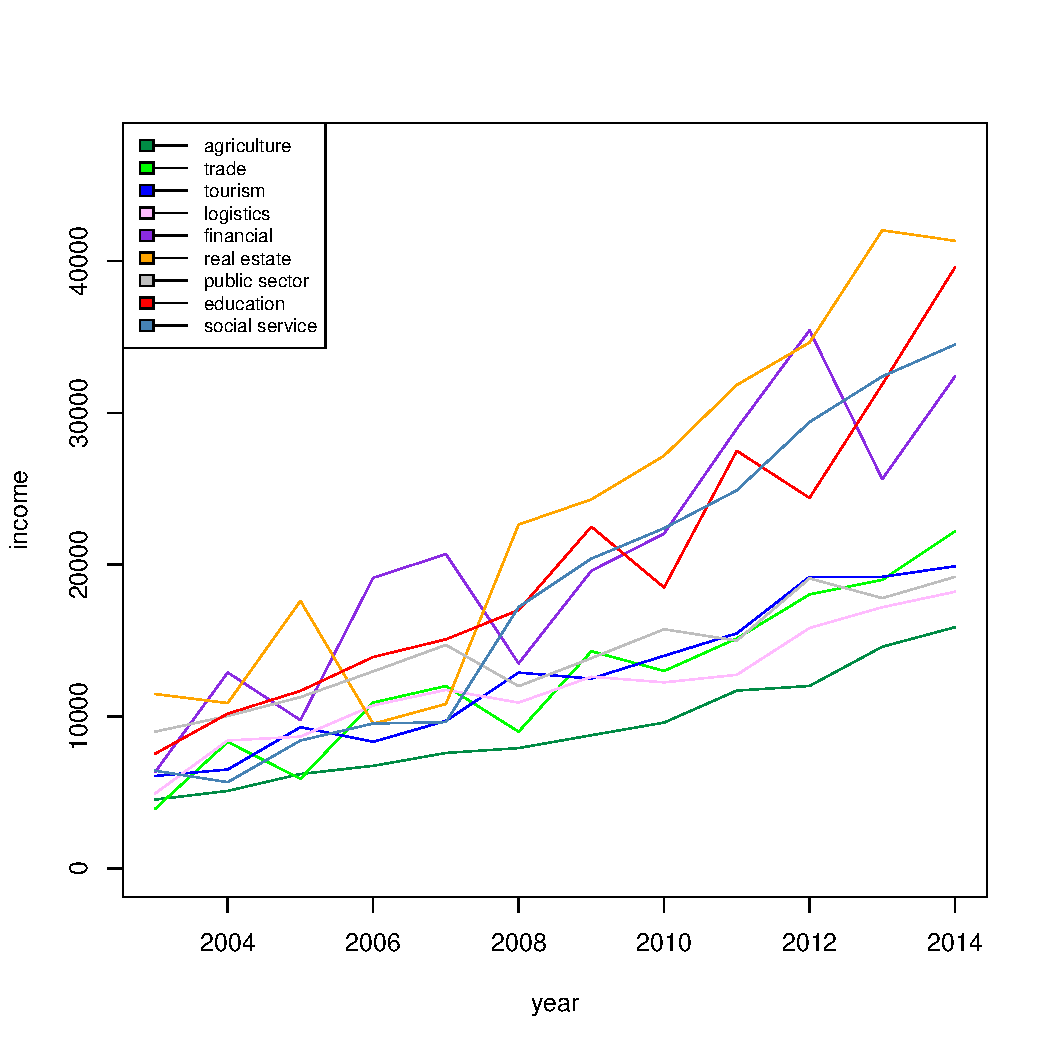
\includegraphics[scale=0.6]{figs/wage2sec.pdf}
	\caption{Historical wage dynamics by sector}
\end{figure}

\begin{table}
	\centering
	\caption{Benchmark Wage to Stock Correlations}
	\begin{tabular}[c]{c|ccc}
		&Low&Moderate&High\\
		\hline
		$\rho_{sw}$&0&0.2&0.4
	\end{tabular}
\end{table}


\paragraph{Individual heterogeneity}

We check for individual heterogeneity using a sensitivity analysis on different risk aversion coefficients, summarized in Table 5.

\begin{table}
	\centering
	\caption{Coefficients of Risk Averion}
	\begin{tabular}[c]{r|cccc}
		Values&Torul&low&default&high\\
		\hline
		$\gamma$&1.5&3&5&10\\
	\end{tabular}
\end{table}

\subsection{Capital series}

\subsubsection{Human capital}
Human capital at all ages has been calculated as a discounted sum of all future wages until retirement with the discount factor $r_f$. To construct the individualized capital we used steep, moderate and flat wage series mentioned in the previous section. It can be seen in Figure 9 that human capital is declining for flat wages and hump-shaped for moderate and steep wages. 

\begin{figure}[h]
	\centering
    \begin{minipage}{0.45\textwidth}
		\centering
		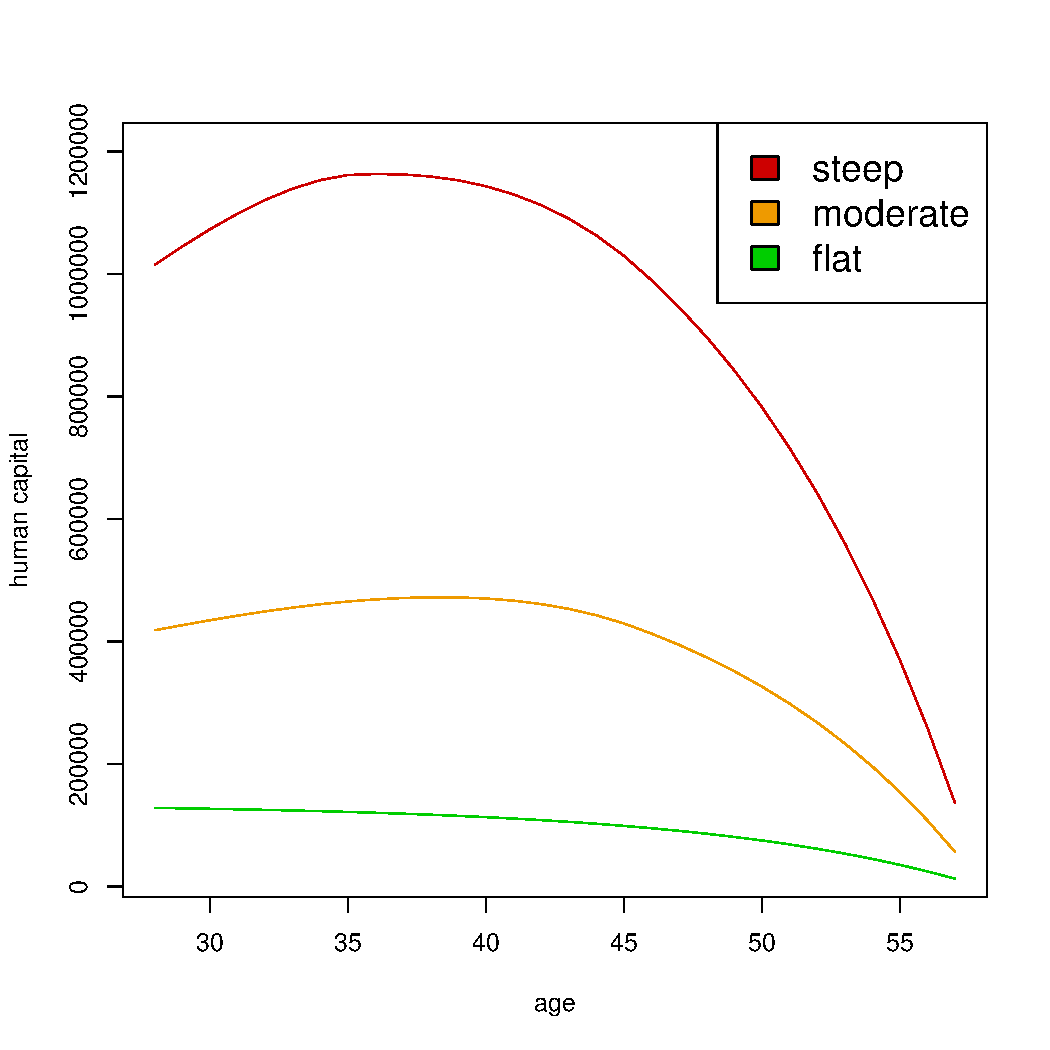
\includegraphics[scale=0.4]{figs/humancapital.pdf}
		\caption{Human capital by age}
	\end{minipage}
	\hfill
    \begin{minipage}{0.45\textwidth}
		\centering
		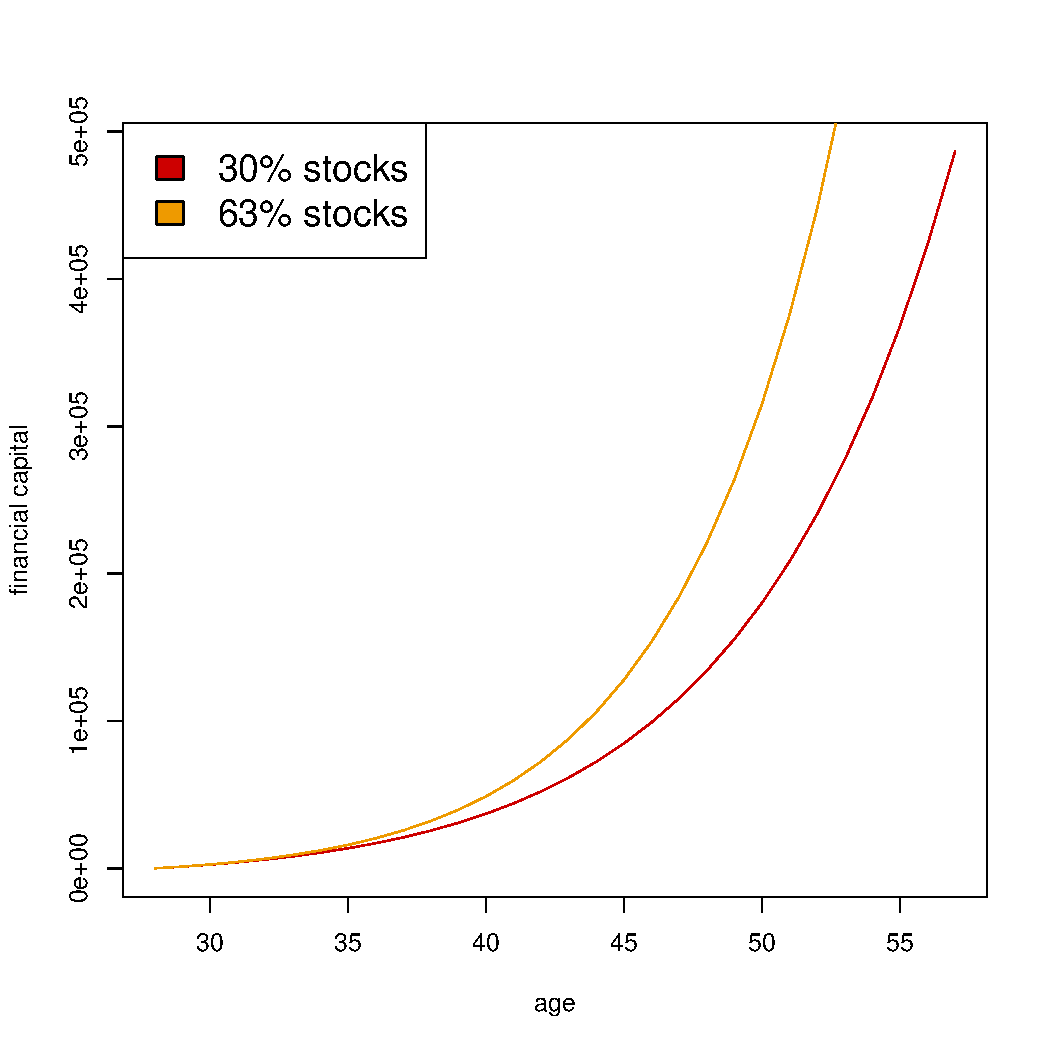
\includegraphics[scale=0.4]{figs/fincapital.pdf}
		\caption{Financial capital by age}
	\end{minipage}
\end{figure}

\subsubsection{Financial capital}

Financial capital evolves according to dynamic investment illustrated in Figure 11. Every period $t$ a certain percentage $c$ (equal to $3\%$ in Turkey) of that period's wage $w_t$ is invested in a retirement portfolio. At the same time, the previously invested amount accrues interest. We started with 28 years old individual who invests for 30 years until retirement, as has been mentioned previously numerous times.

\begin{figure}[h]
	\centering
	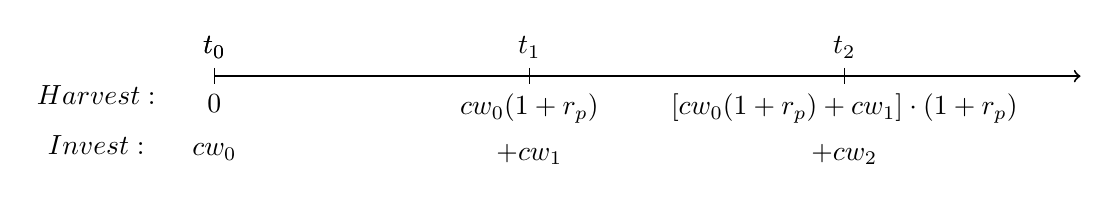
\begin{tikzpicture}
		\draw [->, line width=0.25mm] (0,0) -- (11,0);
		\foreach \x in {0,4,8}
			\draw (\x cm,3pt) -- (\x cm, -3pt);
		\draw (0,0) node[below=21pt] {$ cw_0 $} node[above=3pt] {$ t_0 $};
    	\draw (4,0) node[below=21pt] {$ +cw_1 $} node[above=3pt] {$ t_1 $};
    	\draw (8,0) node[below=21pt] {$ +cw_2 $} node[above=3pt] {$ t_2 $};
		\draw (0,0) node[below=3pt] {$ 0 $} node[above=3pt] {$ t_0 $};
    	\draw (4,0) node[below=3pt] {$ cw_0(1+r_p) $};
    	\draw (8,0) node[below=3pt] {$ \left[cw_0(1+r_p) + cw_1 \right] \cdot (1+r_p) $};
	    \draw (-1.5,0) node[below=18pt] {$ Invest: $};
    	\draw (-1.5,0) node[below=0pt] {$ Harvest: $};
	\end{tikzpicture}
	\caption{Law of motion of financial capital}
\end{figure}

\paragraph{}Note that the shape of the financial capital depends on $r_p$ --- the rate of return on portfolio, which itself depends on the risky-to-riskless asset ratio. Different such ratios are listed and analyzed in detail in the next section. Figure 10 demonstrates the evolution of financial capital for two investment options, provided by Anadolu Hayat Emeklilik --- $30\%$ in stocks and $70\%$ in bonds, and by solving Markowitz's formula --- $63\%$ in stocks and $37\%$ in bonds.

\paragraph{}It is important to notice here that since human capital is declining by age and financial capital is increasing, the ratio $\frac{L_t}{F_t}$ is declining in $t$. Recalling Merton's formula for $\alpha_t$ from Chapter 2, $\frac{\mu - R_f}{\gamma \sigma^2}(1+\frac{L_t}{F_t})$, it should be now clear how the above fraction creates a lifecycle effect --- different ratios for different ages. 

\section{Results}
\label{results}

In this chapter we present the results of our simulation. In the first section we will present the default and individualized lifecycle investment strategies, the former being provided by real retirement funds and the latter being solved by Merton and Munk. We will plug in the heterogeneous parameters, described in detail in the previous chapter. In the next section, we will calculate the resulting financial capital flows and compare their welfare effects using their expected utilities, as mentioned in Chapter 3. 

\subsection{Investment strategies}
\subsubsection{Default lifecyccles}
As was discussed in the previous chapter, our individual decides between investing in risky (stocks) or risk-free (bonds) assets. The default allocations for share of risky asset are given by:

\begin{itemize}
	\item $100-t$, for all $t$
	\item $\begin{cases} 100\%, & t<40\\(200-2.5t)\%, & t\in[40,57]\end{cases}$
	\item $63\%$, for all $t$
	\item $30\%$, for all $t$
\end{itemize}

where the latter two are Markowitz's solution and Anadolu Hayat's moderate investment option respectively. Since we are only interested in age span between 28 and 57, Figure 12 shows the risky asset share $\pi_t$ only for that interval. 

\begin{figure}[h]
	\centering
	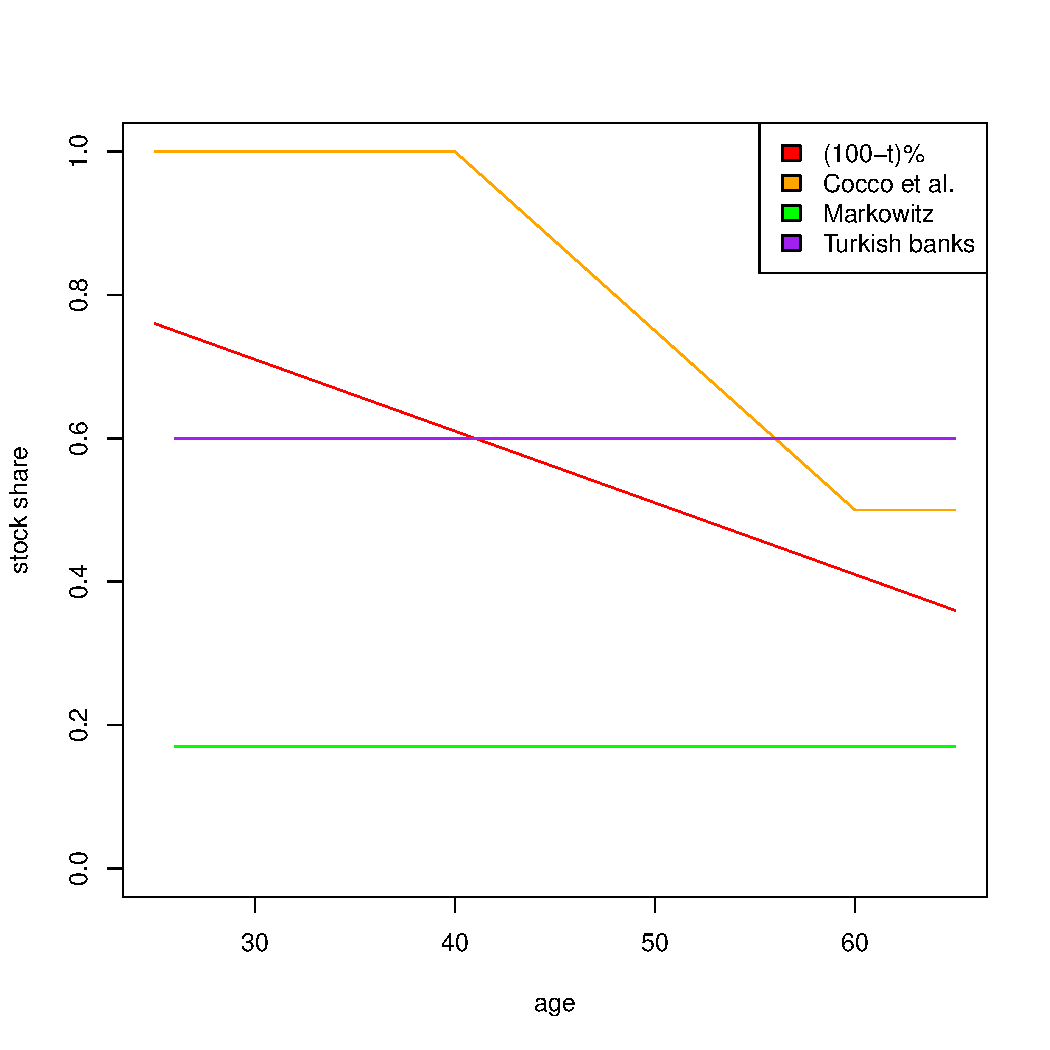
\includegraphics[scale=0.6]{figs/defaults.pdf}
	\caption{Default portfolio allocations of stock investments}
\end{figure}


\subsubsection{Individualized lifecycles}

To derive individualized lifecycle strategies, we used Merton's (1971) and Munk's (2016) optimal portfolio allocation formulas mentioned in chapters 2 and 3. Since these formulas depended on intratemporal amounts of capital, we have constructed three human capital series corresponding to flat, moderate and steep wage growth curves mentioned in the previous chapter. Figure 13 illustrates the risky asset shares given by Merton and Munk without housing for various levels of labor income growth and risk aversion. The figure shows that the steeper the wage growth curves get or the lower their risk aversion is, the more aggressive investors are. However, as a whole, they follow the similar pattern. The figure also shows that for small correlations between labor income and stock prices, Munk's solution converges to Merton's solution, as was shown in Chapter 3.

\begin{figure}
	\centering
    \begin{subfigure}{0.45\textwidth}
		\centering
		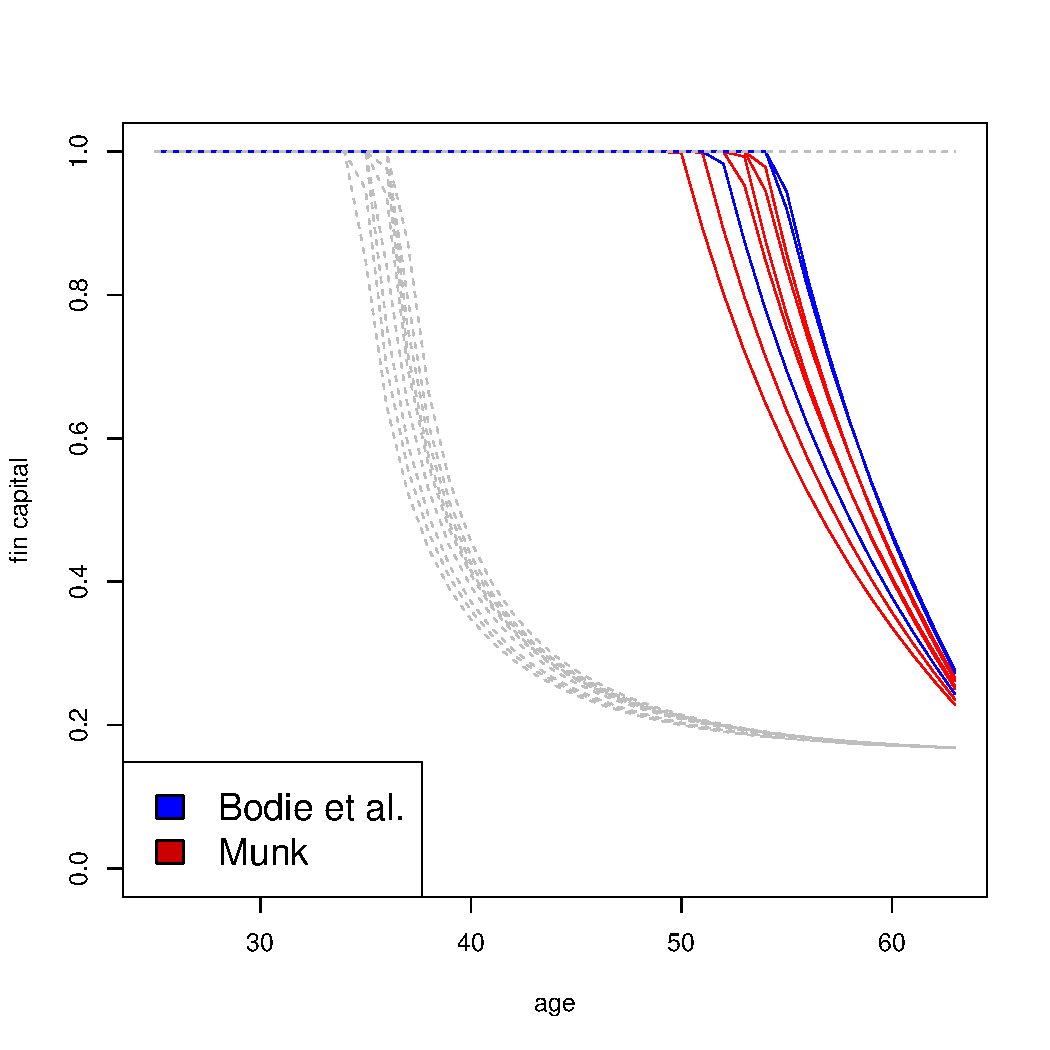
\includegraphics[scale=0.4]{figs/individuals15.pdf}
		\caption{$\gamma = 1.5$}
	\end{subfigure}
	\hfill
    \begin{subfigure}{0.45\textwidth}
		\centering
		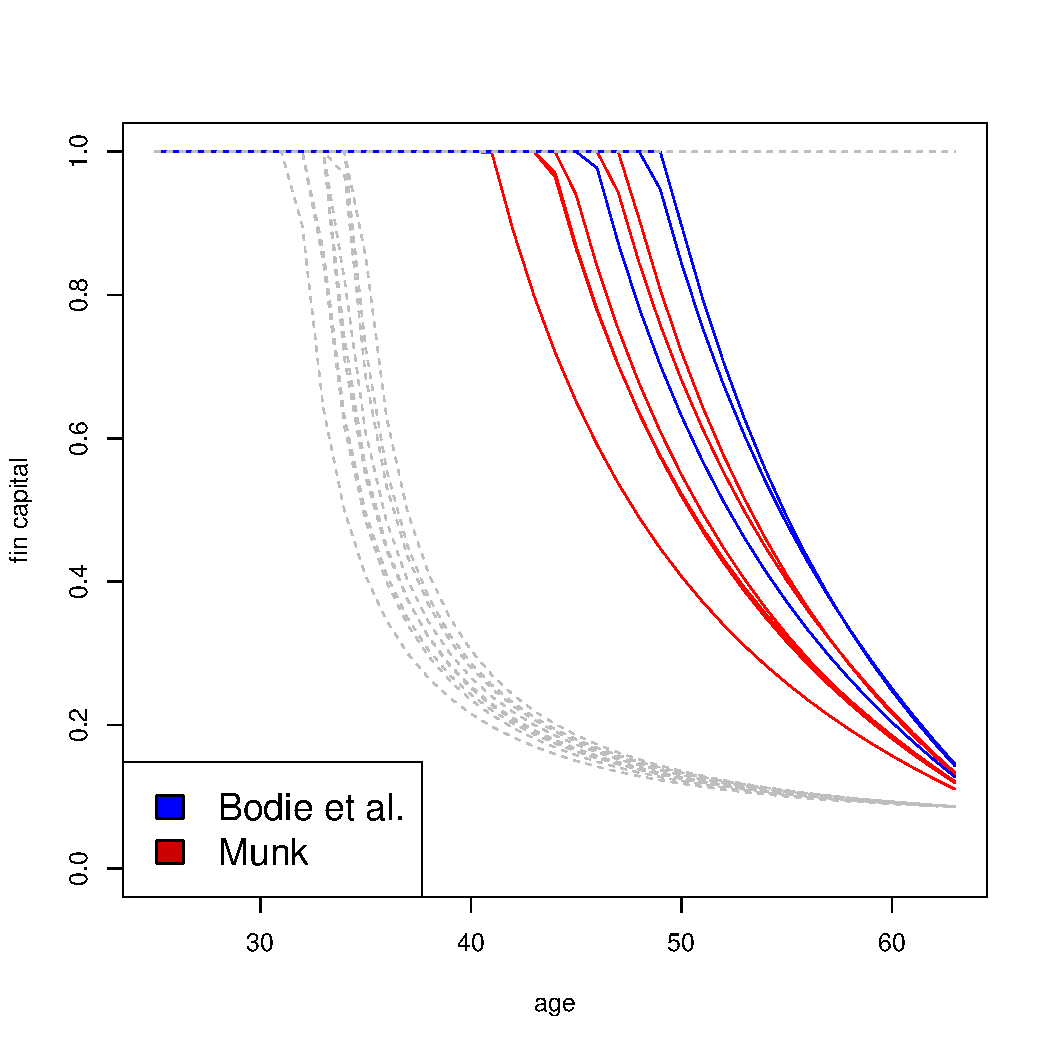
\includegraphics[scale=0.4]{figs/individuals3.pdf}
		\caption{$\gamma = 3$}
	\end{subfigure}
	\hfill
    \begin{subfigure}{0.45\textwidth}
		\centering
		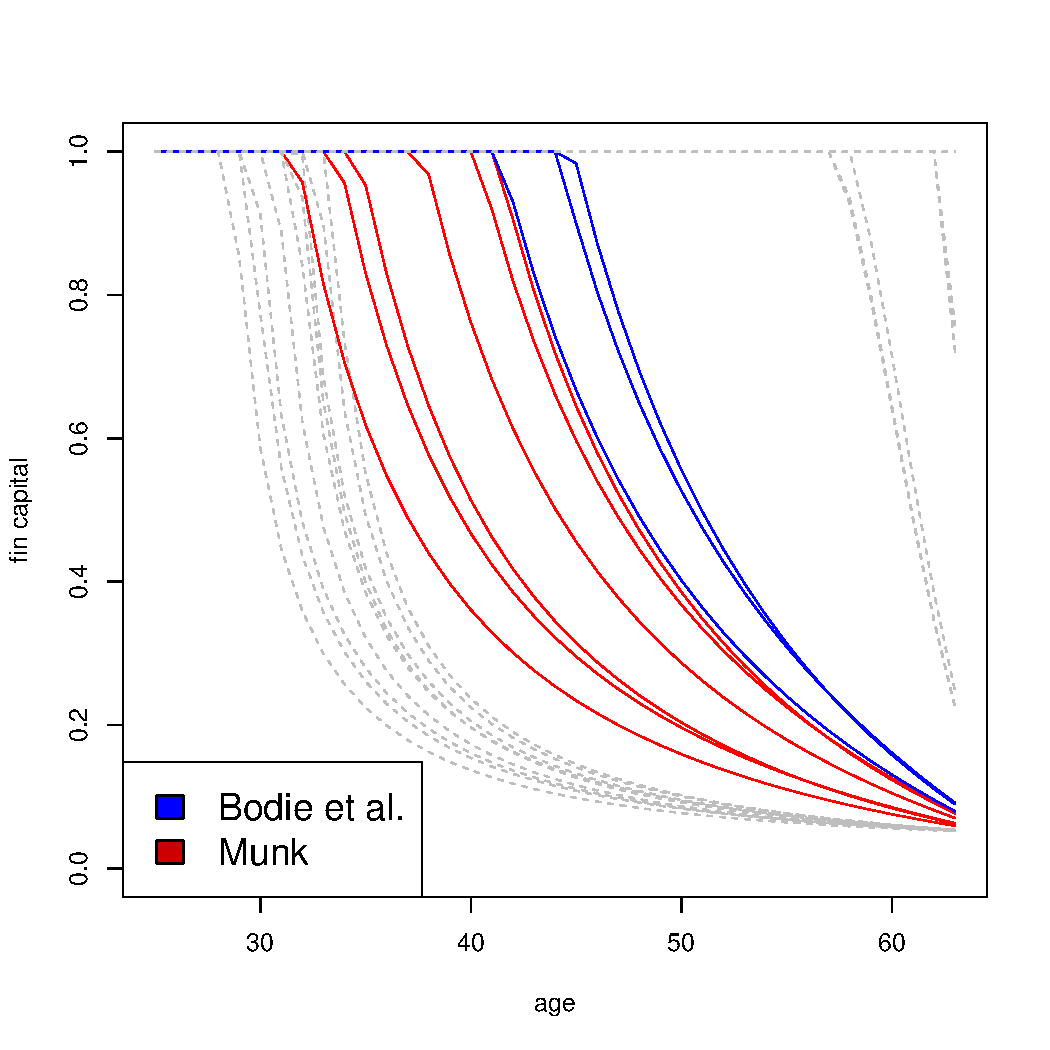
\includegraphics[scale=0.4]{figs/individuals5.pdf}
		\caption{$\gamma = 5$}
	\end{subfigure}
	\hfill
    \begin{subfigure}{0.45\textwidth}
		\centering
		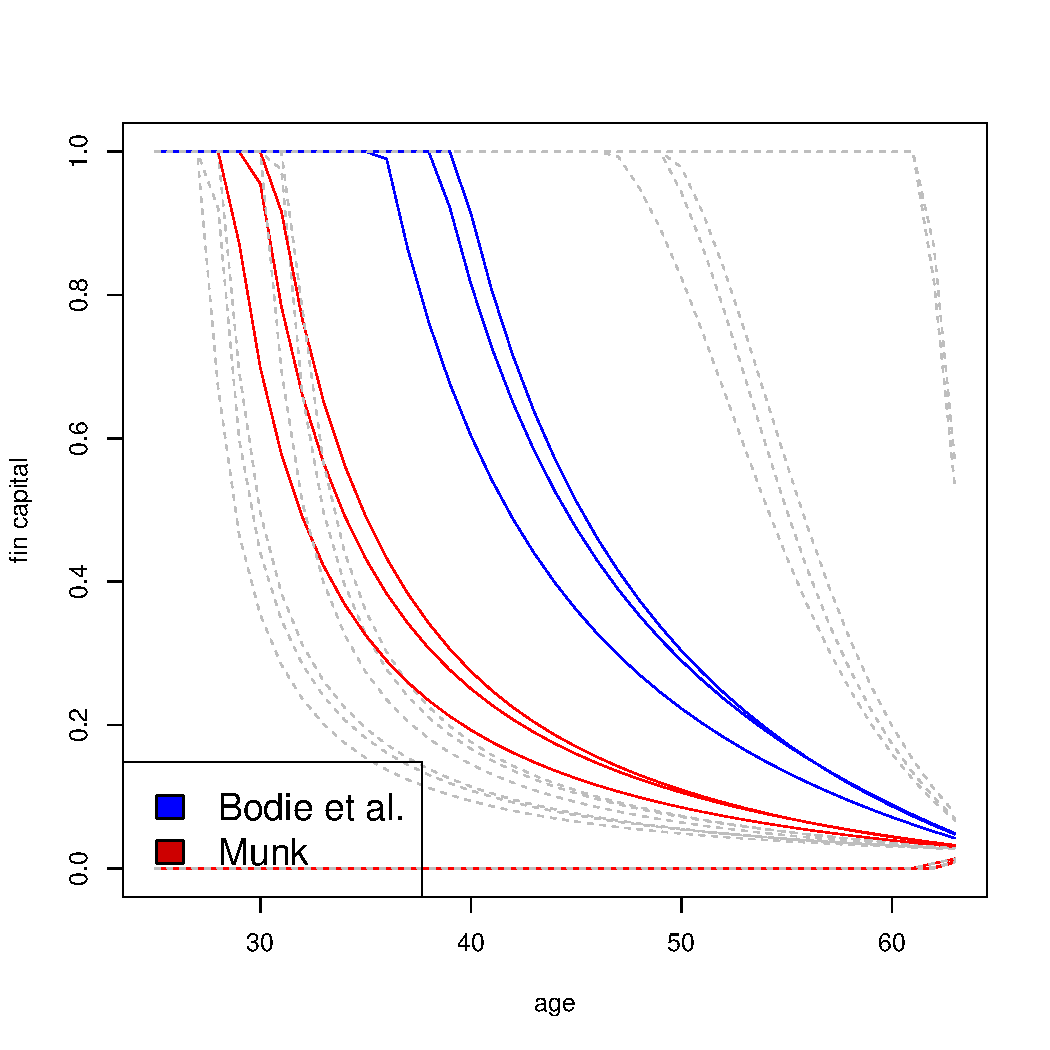
\includegraphics[scale=0.4]{figs/individuals10.pdf}
		\caption{$\gamma = 10$}
	\end{subfigure}
	\caption{Merton and Munk's solution without housing for different wage growth and risk aversion levels}
\end{figure}

\paragraph{}Figure 14 illustrates the stock and housing asset shares determined by Munk with housing for flat, moderate and steep labor income curves and low, moderate and high stock-labor income correlations for different levels of risk aversion, to capture heterogeneity, as mentioned in the previous chapter. The figure confirms that steeper labor income curves result in larger share of stocks in portfolio and less of bonds. Around age of 45, the sum of optimal stock and housing investments falls below $1$ and optimal bond investment becomes positive. Also, the higher the risk aversion, the less the individuals want to invest in both housing and stocks --- for $\gamma=10$, the optimal Munk solutions are negative or add up to less than $1$, meaning that they should sell all stocks and housing to invest in risk-free long term bonds. In our analysis we do not allow for negative investing, since this is not a primary focus of our paper.  



\paragraph{}Full tables with actual solutions are available in Tables 9 and 10 of Appendix E for models without housing and in Table 10 for a model with housing. 


\subsection{Welfare comparison}

In order to compare welfare we use CRRA expected utility function, mentioned in Chapter 3. The probabilities of survival are taken from TUIK as mentioned in the previous chapter. The consumption is calculated in numbers of consumption baskets which cost exactly $1$ CPI --- consumer price index at that period, which is increasing with inflation rate annually, and is equal to $100$ at retirement age $57$. The wealth for which consumption baskets are purchased is a total accumulated wealth, including stock returns, bond returns and housing returns, annuitized according to the formula described in Chapter 3. Discount rate is $0.89$, as mentioned in the previous chapter. We compare expected utilities for different levels of risk aversion.

\begin{figure}[H]
	\centering
    \begin{subfigure}{0.45\textwidth}
		\centering
		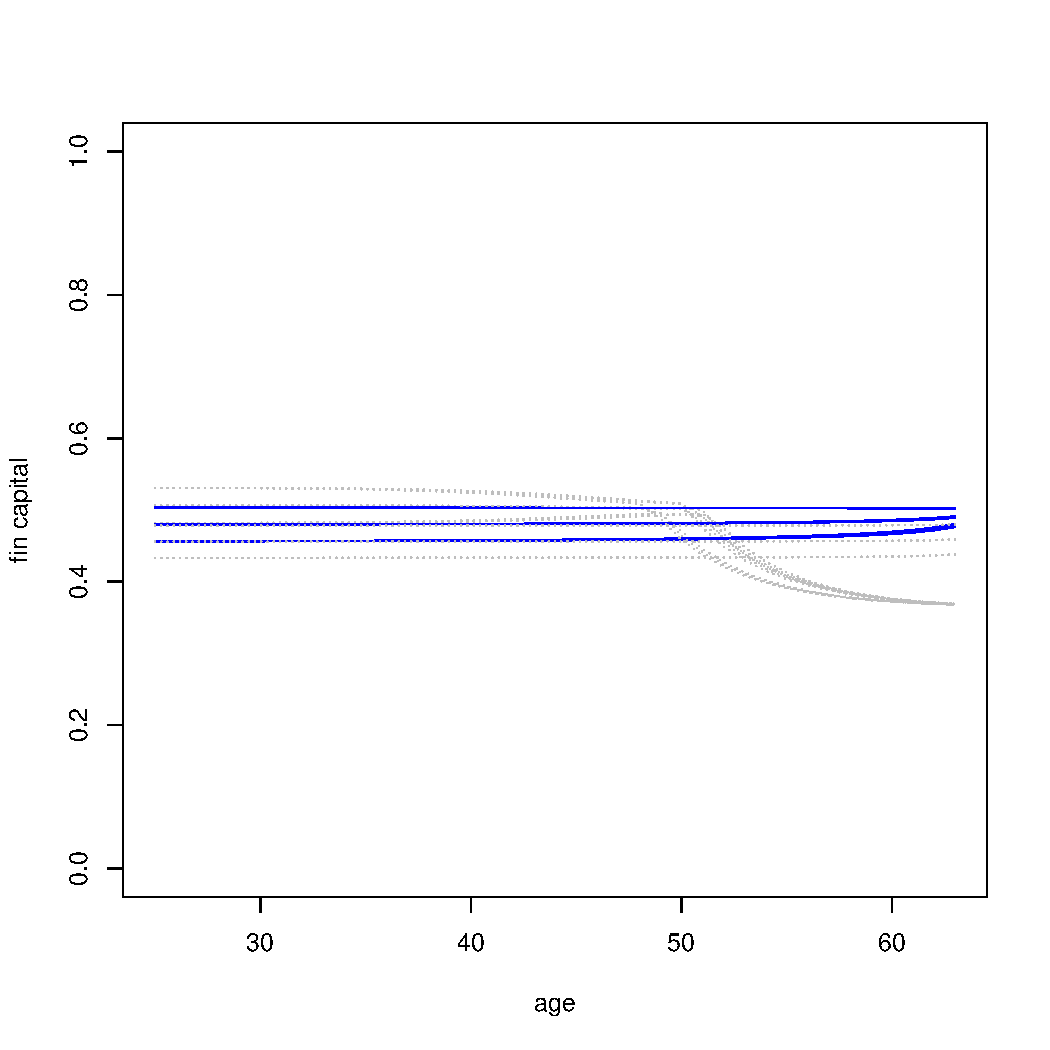
\includegraphics[scale=0.4]{figs/smunkhouse15.pdf}
		\caption{Stocks for $\gamma = 1.5$}
	\end{subfigure}
	\hfill
    \begin{subfigure}{0.45\textwidth}
		\centering
		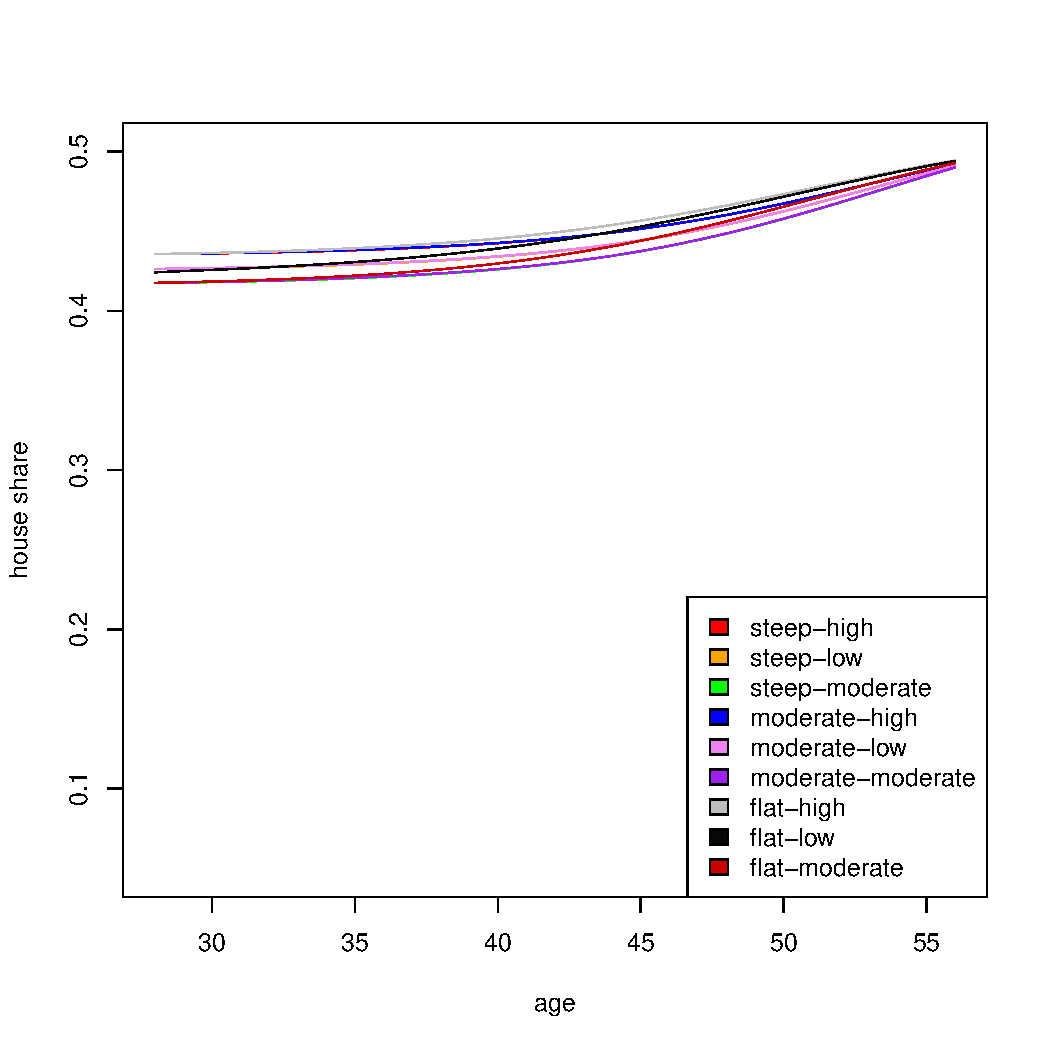
\includegraphics[scale=0.4]{figs/hmunkhouse15.pdf}
		\caption{Housing for $\gamma = 1.5$}
	\end{subfigure}
	\hfill
    \begin{subfigure}{0.45\textwidth}
		\centering
		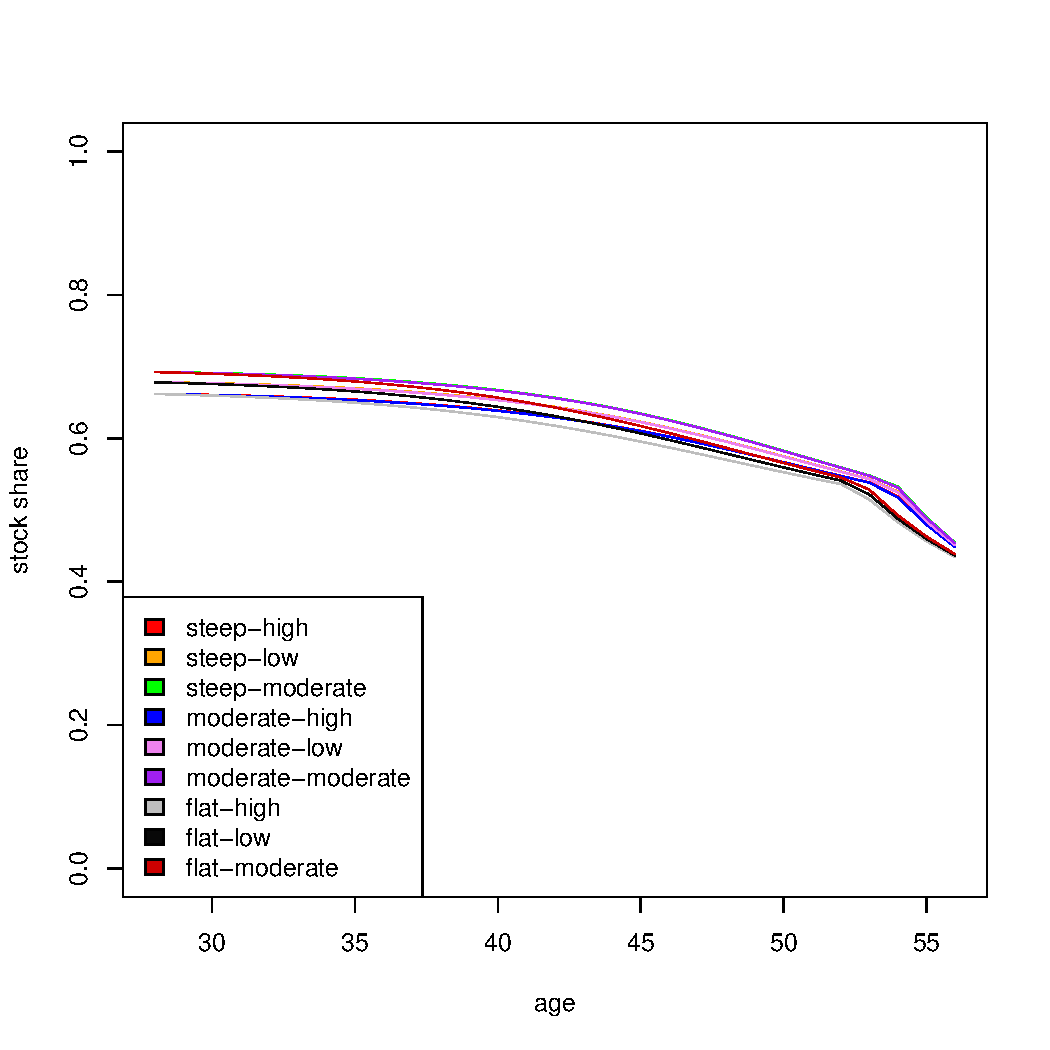
\includegraphics[scale=0.4]{figs/smunkhouse3.pdf}
		\caption{Stocks for $\gamma = 3$}
	\end{subfigure}
	\hfill
    \begin{subfigure}{0.45\textwidth}
		\centering
		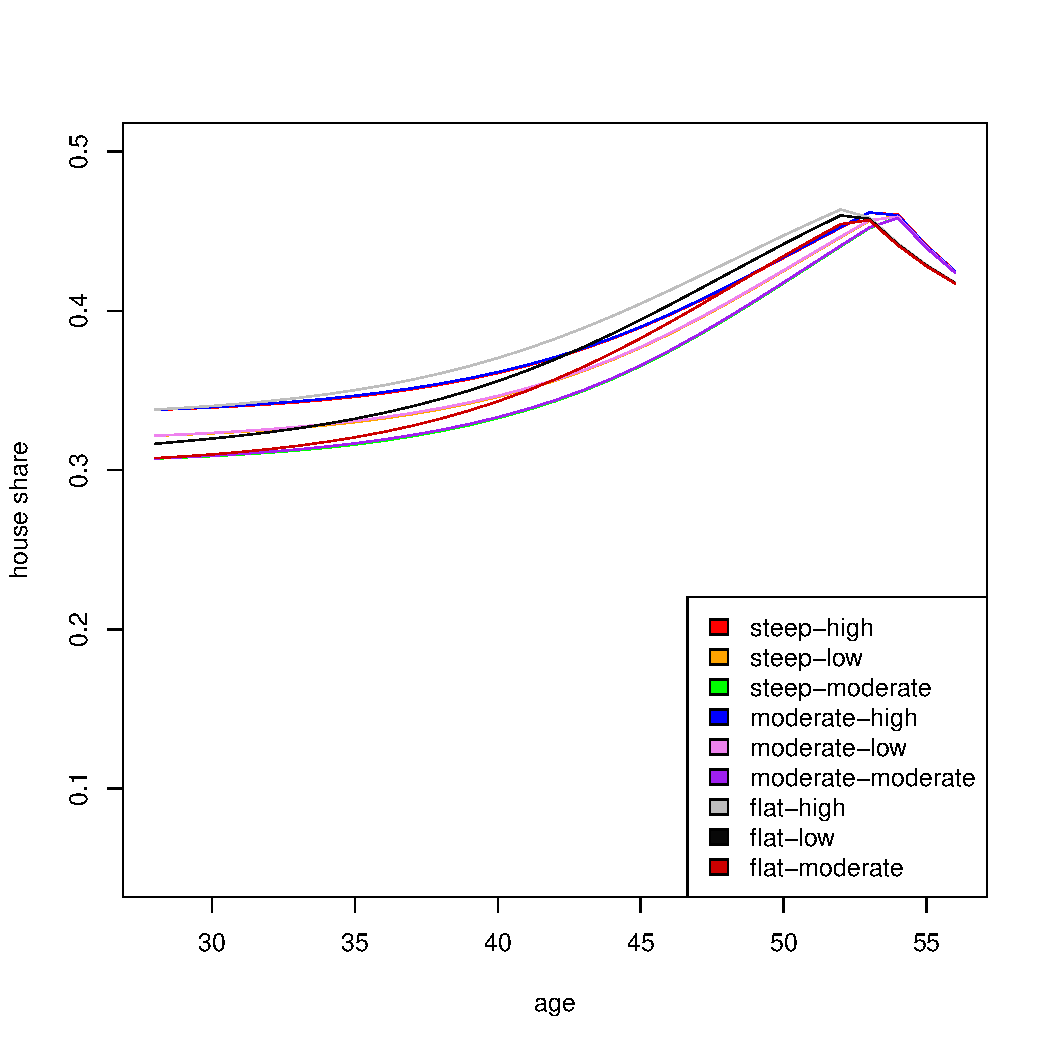
\includegraphics[scale=0.4]{figs/hmunkhouse3.pdf}
		\caption{Housing for $\gamma = 3$}
	\end{subfigure}
	\hfill
    \begin{subfigure}{0.45\textwidth}
		\centering
		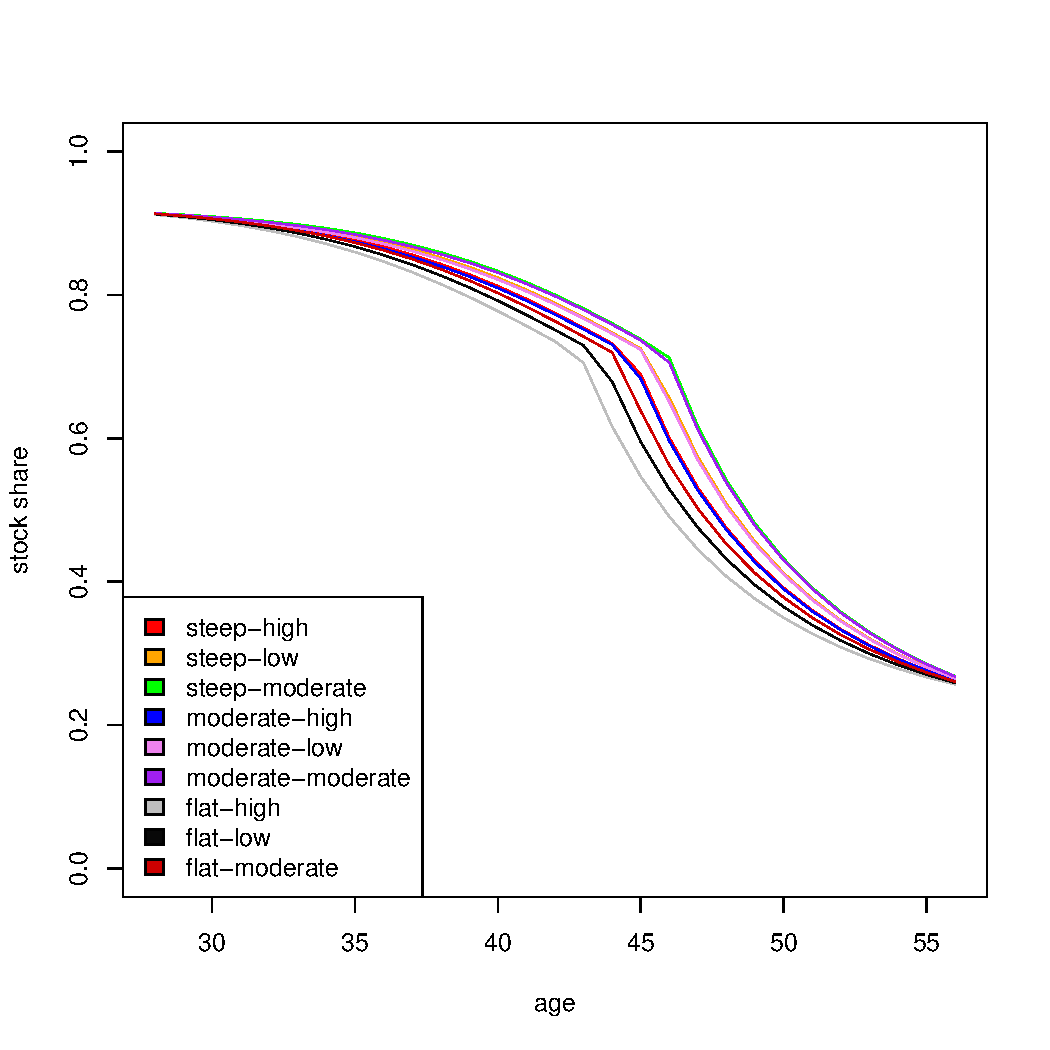
\includegraphics[scale=0.4]{figs/smunkhouse5.pdf}
		\caption{Stocks for $\gamma = 5$}
	\end{subfigure}
	\hfill
    \begin{subfigure}{0.45\textwidth}
		\centering
		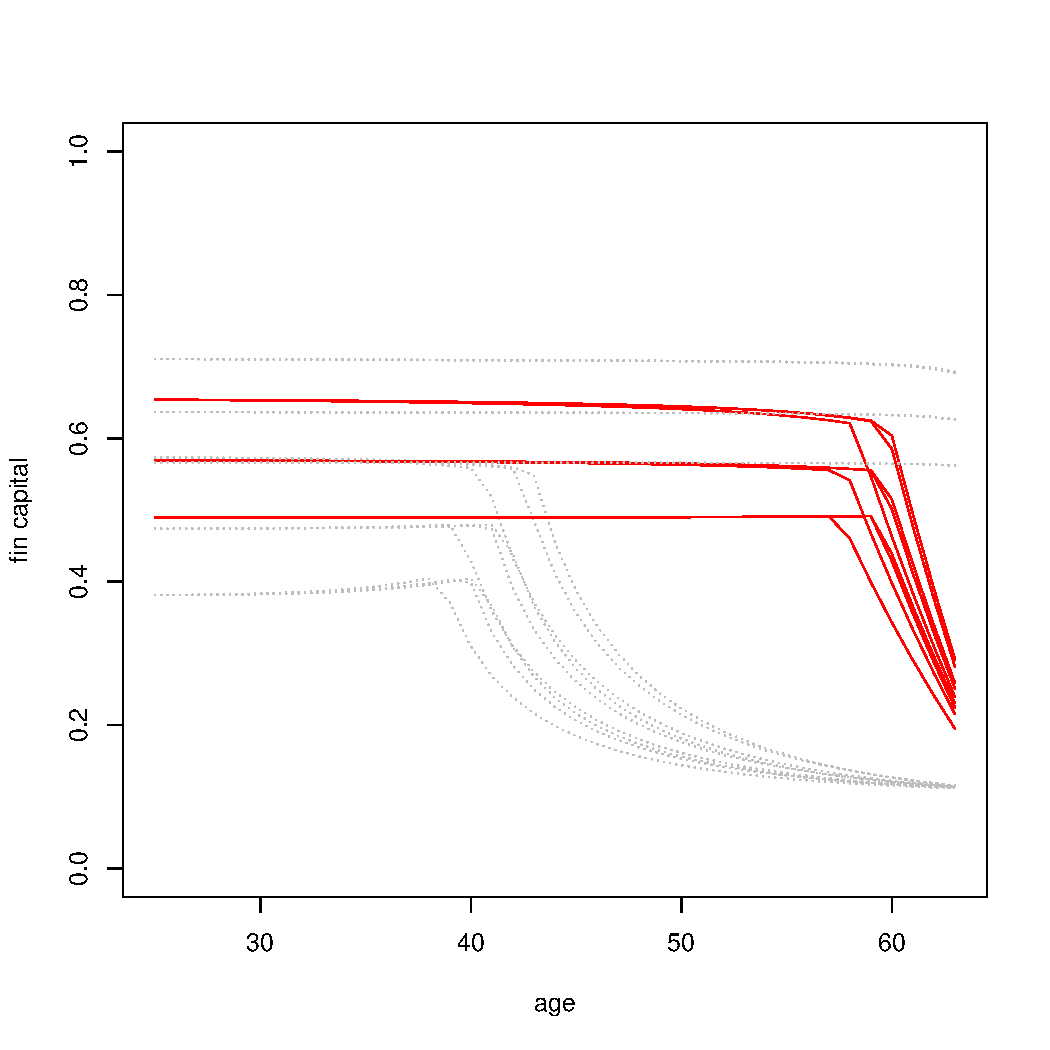
\includegraphics[scale=0.4]{figs/hmunkhouse5.pdf}
		\caption{Housing for $\gamma = 5$}
	\end{subfigure}
\end{figure}
\begin{figure}[H]\ContinuedFloat
    \begin{subfigure}{0.45\textwidth}
		\centering
		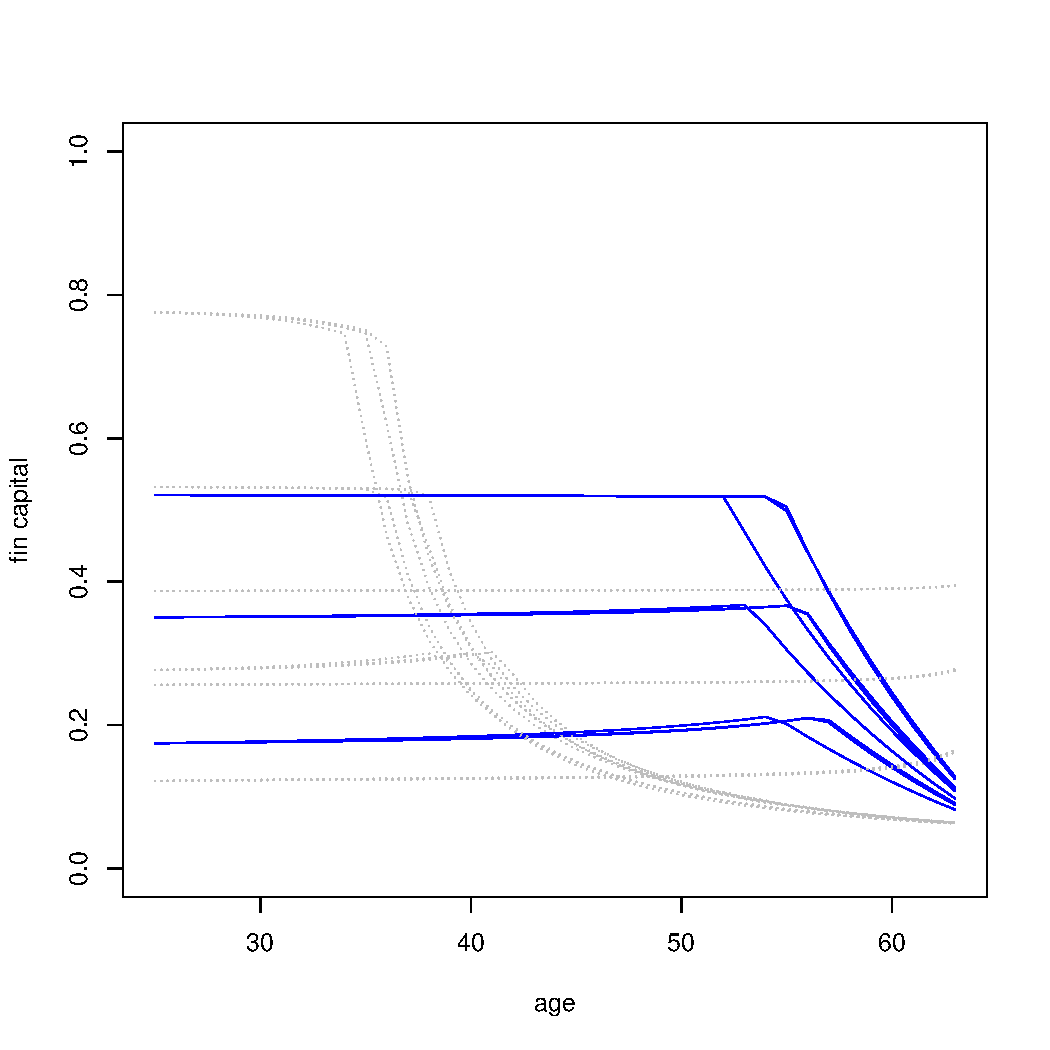
\includegraphics[scale=0.4]{figs/smunkhouse10.pdf}
		\caption{Stocks for $\gamma = 10$}
	\end{subfigure}
	\hfill
    \begin{subfigure}{0.45\textwidth}
		\centering
		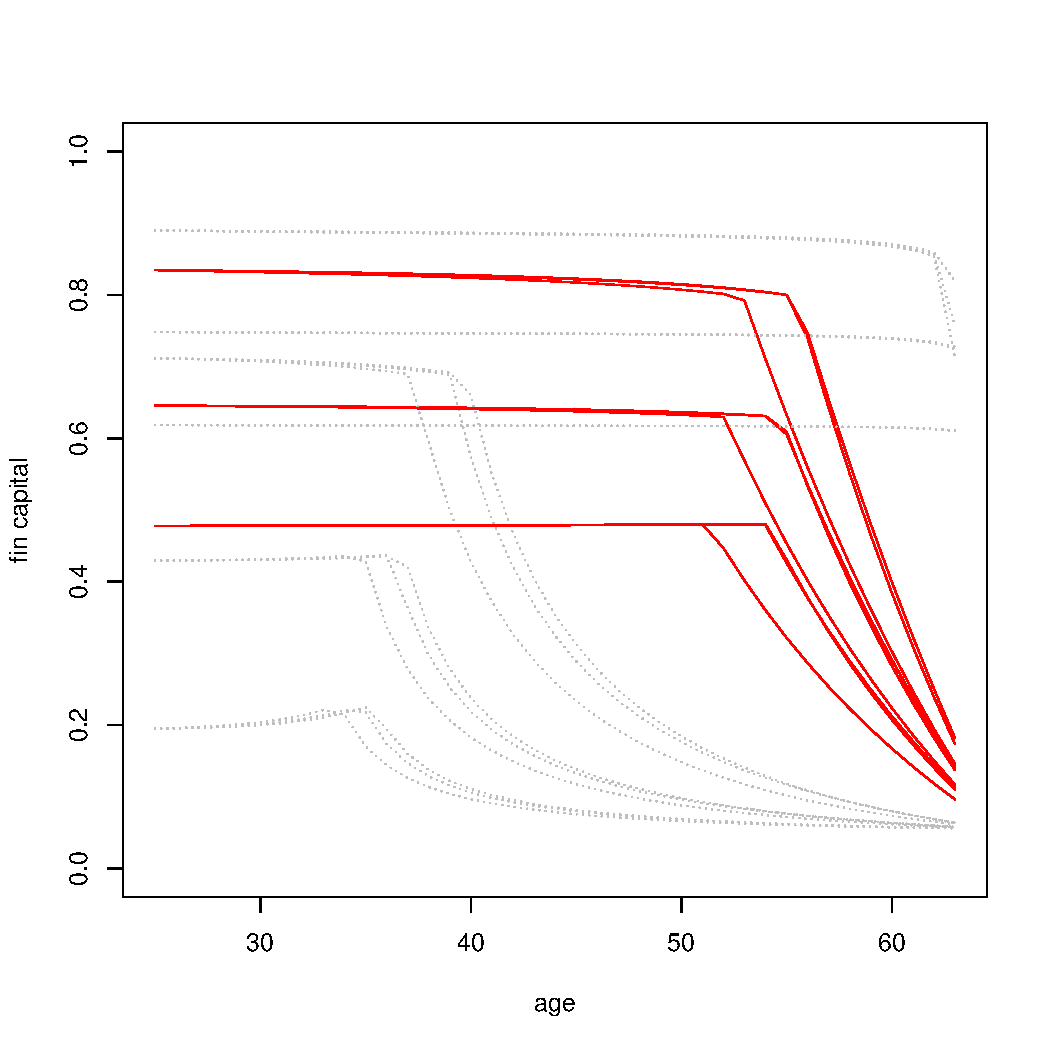
\includegraphics[scale=0.4]{figs/hmunkhouse10.pdf}
		\caption{Housing for $\gamma = 10$}
	\end{subfigure}
	\caption{Munk's stock and housing shares for different wage growth, stock-wage correlation and risk aversion levels}
\end{figure}

\subsubsection{Early results}

After a lifetime of investing in the above portfolios, the household accumulates different levels of wealth, summarized in Table 6. Since the consumption preferences are monotonic, we can make early conclusions even without calculating expected utilities --- the higher the accumulated wealth, the better: 

\begin{itemize}
\item Naively considering lifecycles does not guarantee the better investment. So, in our case, $(100-age)\%$ is worse than fixed Markowitz.
\item Different stock-wage correlations don't make much difference in the outcome without housing, and make considerable difference in models with housing
\item Stock-wage correlations are negatively correlated with total wealth
\item Both too low and too high risk aversion results in less accumulated capital than moderate risk aversion for models with housing and only too high risk aversion --- for models without housing (because of monotonicity).\\
\item Default options are better for people with flat wage growth rate and worse for people with moderate or steep wage curves
\end{itemize}

\subsubsection{Annuitization}
To formalize the observations made in the previous section, we will construct annuities and plug them into expected utility functions. As described in detail in Chapter 3, we define annuities by dividing the total wealth before retirement by the discount factor $1 + \sum^{100}_{t=58}\frac{p_t}{1+r_f}$. Using survival probabilities, obtained from TUIK, and risk-free rate of return, described in the previous chapter, we calculate the discount factor as $205.29$. The annuities are obtained by dividing all the values in the Table 6 by $205.29$. The resulting values are presented in Table 7. 


\subsubsection{Consumption during retirement}
We model that the individuals spend their annuity returns to consume baskets which cost $100$ TL during the year, when our agent is 58 years old, and increase by inflation rate $\pi = 8.4\%$. Thus, every period $t>57$ our agent consumes $\frac{annuity}{100\cdot\left(1.084\right)^{t-58}}$. We do not provide the separate table with the value streams, as they will be implicitly included in utility values.


\subsubsection{Expected utilities}
Finally, we will plug the consumption streams, calculated in the previous section, into the constant relative risk-aversion expected utility functions to compare the welfare effects. The resulting expected utility values are presented in Table 8.


\newgeometry{top=2cm,bottom=2cm}
\begin{table}%TABLE 5.1
	\centering
	\caption{Total Accumulated Wealth by Investment Option}
	\begin{tabular}[c]{lrrrr}
		\hline
		Option&$\gamma=5$ (default) & $\gamma=1.5$ & $\gamma=3$ & $\gamma=10$\\
		\hline
		\multicolumn{5}{c}{Defaults}\\
Anadolu Hayat (riskless)&614,195 TL&614,195 TL&614,195 TL&614,195 TL\\
$(100-age)\%$&1,160,977 TL&1,160,977 TL&1,160,977 TL&1,160,977 TL\\
Cocco et al.&1,599,852 TL&1,599,852 TL&1,599,852 TL&1,599,852 TL\\
Markowitz&1,300,187 TL&1,300,187 TL&1,300,187 TL&1,300,187 TL\\
\multicolumn{5}{c}{}\\
\multicolumn{5}{c}{Individualized (no housing)}\\
Merton (steep)&3,812,053 TL&4,212,735 TL&3,104,746 TL&2,920,892 TL\\
Merton (moderate)&1,629,904 TL&1,813,821 TL&1,447,951 TL&1,248,330 TL\\
Merton (flat)&543,602 TL&612,548 TL&639,866 TL&398,235 TL\\
Munk (steep-lo)&3,547,442 TL&4,168,823 TL&3,829,218 TL&2,085,883 TL\\
Munk (steep-mod)&3,543,435 TL&4,164,850 TL&3,825,221 TL&2,081,872 TL\\
Munk (steep-hi)&3,539,425 TL&4,160,872 TL&3,821,219 TL&2,077,854 TL\\
Munk (moderate-lo)&1,513,198 TL&1,794,772 TL&1,689,491 TL&868,955 TL\\
Munk (moderate-mod)&1,511,527 TL&1,793,113 TL&1,687,822 TL&867,281 TL\\
Munk (moderate-hi)&1,509,853 TL&1,791,452 TL&1,686,152 TL&865,604 TL\\
Munk (flat-lo)&508,757 TL&606,410 TL&657,762 TL&262,161 TL\\
Munk (flat-mod)&508,371 TL&606,025 TL&657,376 TL&261,774 TL\\
Munk (flat-hi)&507,984 TL&605,640 TL&656,990 TL&261,386 TL\\
\multicolumn{5}{c}{}\\
\multicolumn{5}{c}{Individualized (no housing)}\\
Munk (steep-lo)&8,937,159 TL&3,087,377 TL&4,718,332 TL&3,920,863 TL\\
Munk (steep-mod)&7,645,621 TL&2,966,467 TL&4,371,031 TL&2,900,022 TL\\
Munk (steep-hi)&6,353,327 TL&2,846,577 TL&4,017,054 TL&1,872,799 TL\\
Munk (moderate-lo)&3,652,223 TL&1,304,014 TL&1,998,234 TL&1,605,470 TL\\
Munk (moderate-mod)&3,125,930 TL&1,252,432 TL&1,850,278 TL&1,189,240 TL\\
Munk (moderate-hi)&2,599,301 TL&1,201,297 TL&1,700,235 TL&770,295 TL\\
Munk (flat-lo)&1,026,845 TL&430,353 TL&614,929 TL&455,296 TL\\
Munk (flat-mod)&881,934 TL&435,168 TL&598,789 TL&341,199 TL\\
Munk (flat-hi)&736,896 TL&397,829 TL&527,533 TL&226,188 TL\\
		\hline
	\end{tabular}
\end{table}
\resetgeometry


\newgeometry{top=2cm,bottom=2cm}
\begin{table}%TABLE 5.2
	\centering
	\caption{Annual Pensions by Investment Option}
	\begin{tabular}[c]{lrrrr}
		\hline
		Option&$\gamma=5$ (default) & $\gamma=1.5$ & $\gamma=3$ & $\gamma=10$\\
		\hline
		\multicolumn{5}{c}{Defaults}\\
Anadolu Hayat (riskless) TL&2,992 TL&2,992 TL&2,992 TL&2,992 TL\\
$(100-age)\%$ TL&5,655 TL&5,655 TL&5,655 TL&5,655 TL\\
Cocco et al. TL&7,793 TL&7,793 TL&7,793 TL&7,793 TL\\
Markowitz TL&6,333 TL&6,333 TL&6,333 TL&6,333 TL\\
\multicolumn{5}{c}{}\\
\multicolumn{5}{c}{Individualized (no housing)}\\
Merton (steep) TL&18,569 TL&20,521 TL&15,124 TL&14,228 TL\\
Merton (moderate) TL&7,940 TL&8,835 TL&7,053 TL&6,081 TL\\
Merton (flat) TL&2,648 TL&2,984 TL&3,117 TL&1,940 TL\\
Munk (steep-lo) TL&17,280 TL&20,307 TL&18,653 TL&10,161 TL\\
Munk (steep-mod) TL&17,261 TL&20,288 TL&18,633 TL&10,141 TL\\
Munk (steep-hi) TL&17,241 TL&20,268 TL&18,614 TL&10,122 TL\\
Munk (moderate-lo) TL&7,371 TL&8,743 TL&8,230 TL&4,233 TL\\
Munk (moderate-mod) TL&7,363 TL&8,735 TL&8,222 TL&4,225 TL\\
Munk (moderate-hi) TL&7,355 TL&8,726 TL&8,214 TL&4,216 TL\\
Munk (flat-lo) TL&2,478 TL&2,954 TL&3,204 TL&1,277 TL\\
Munk (flat-mod) TL&2,476 TL&2,952 TL&3,202 TL&1,275 TL\\
Munk (flat-hi) TL&2,474 TL&2,950 TL&3,200 TL&1,273 TL\\
\multicolumn{5}{c}{}\\
\multicolumn{5}{c}{Individualized (housing)}\\
Munk (steep-lo) TL&43,534 TL&15,039 TL&22,984 TL&19,099 TL\\
Munk (steep-mod) TL&37,243 TL&14,450 TL&21,292 TL&14,126 TL\\
Munk (steep-hi) TL&30,948 TL&13,866 TL&19,568 TL&9,123 TL\\
Munk (moderate-lo) TL&17,791 TL&6,352 TL&9,734 TL&7,820 TL\\
Munk (moderate-mod) TL&15,227 TL&6,101 TL&9,013 TL&5,793 TL\\
Munk (moderate-hi) TL&12,662 TL&5,852 TL&8,282 TL&3,752 TL\\
Munk (flat-lo) TL&5,002 TL&2,096 TL&2,995 TL&2,218 TL\\
Munk (flat-mod) TL&4,296 TL&2,120 TL&2,917 TL&1,662 TL\\
Munk (flat-hi) TL&3,590 TL&1,938 TL&2,570 TL&1,102 TL\\

		\hline
	\end{tabular}
\end{table}
\resetgeometry

\subsection{Conclusions}
Now, we can observe the final resutls:

\begin{itemize}

\item Naive lifecycle investment portfolios, such as $(100-age)\%$ don't overperform fixed-ratio Markowitz, because they don't take the risk aversion into consideration.
\item Cocco et al.'s $(200-2.5\cdot age)\%$ approximation is the best default portfolio. It is easy to interpret and captures lifecycle effect.
\item All models perform better for higher risk aversion and worse for lower risk aversion --- for everyone except flat-wagers.
\item Higher stock-wage correlation considerably decreases the utility for moderate and flat wages, and doesn't affect much for steep wages.
\item Merton's solution outperforms Munk's solution without housing for low levels of risk aversion, and performs same for high level of risk aversion ($\gamma=10$).
\item Munk's solution with housing outperforms every other solution for high levels of risk aversion ($\gamma=10$) --- for everyone except flat-wagers.
\item Munk's solution with housing outperforms Munk's solution without housing for $\gamma=5,10$.
\item Markowitz's solution outperforms both Merton's and Munk's solutions for flat wages and low risk aversion.
\item Individualizing lifecycles by wage growth rate and stock-wage correlation increases welfare for steep wagers and decreases welfare for flat wagers.
\end{itemize}

\paragraph{}We did not provide numerical conclusions, since they are trivial --- they can be obtained by calculating percentage differences in Table 8.

\newgeometry{top=2cm,bottom=2cm}
\begin{table}%TABLE 5.3
	\centering
	\caption{Expected Utilities by Investment Option}
	\begin{tabular}[c]{lrrrr}
		\hline
		Option&$\gamma=5$ (default) & $\gamma=1.5$ & $\gamma=3$ & $\gamma=10$\\
		\hline
\multicolumn{5}{c}{Defaults}\\
Anadolu Hayat (riskless)&-0.0008389&-3.6004130&-0.0247934&-0.0000509\\
(100-age)\%&-0.0000657&-2.6187470&-0.0069390&-0.0000002\\
Cocco et al.&-0.0000182&-2.2308240&-0.0036542&0.0000000\\
Markowitz&-0.0000418&-2.4745850&-0.0055327&-0.0000001\\
\multicolumn{5}{c}{}\\
\multicolumn{5}{c}{Individualized (no housing)}\\
Merton (steep)&-0.0000006&-1.3747480&-0.0009703&0.0000000\\
Merton (moderate)&-0.0000169&-2.0951160&-0.0044611&-0.0000001\\
Merton (flat)&-0.0013672&-3.6052480&-0.0228439&-0.0025138\\
Munk (steep-lo)&-0.0000008&-1.3819700&-0.0006379&0.0000000\\
Munk (steep-mod)&-0.0000008&-1.3826290&-0.0006392&0.0000000\\
Munk (steep-hi)&-0.0000008&-1.3832900&-0.0006405&0.0000000\\
Munk (moderate-lo)&-0.0000228&-2.1062050&-0.0032767&-0.0000022\\
Munk (moderate-mod)&-0.0000229&-2.1071790&-0.0032832&-0.0000023\\
Munk (moderate-hi)&-0.0000230&-2.1081550&-0.0032897&-0.0000023\\
Munk (flat-lo)&-0.0017820&-3.6234500&-0.0216177&-0.1082611\\
Munk (flat-mod)&-0.0017874&-3.6245990&-0.0216431&-0.1097095\\
Munk (flat-hi)&-0.0017929&-3.6257500&-0.0216686&-0.1111816\\
\multicolumn{5}{c}{}\\
\multicolumn{5}{c}{Individualized (housing)}\\
Munk (steep-lo)&0.0000000&-1.6058700&-0.0004201&0.0000000\\
Munk (steep-mod)&0.0000000&-1.6382700&-0.0004895&0.0000000\\
Munk (steep-hi)&-0.0000001&-1.6724140&-0.0005796&0.0000000\\
Munk (moderate-lo)&-0.0000007&-2.4709510&-0.0023424&0.0000000\\
Munk (moderate-mod)&-0.0000013&-2.5213210&-0.0027320&-0.0000001\\
Munk (moderate-hi)&-0.0000026&-2.5744240&-0.0032354&-0.0000066\\
Munk (flat-lo)&-0.0001074&-4.3012340&-0.0247341&-0.0007532\\
Munk (flat-mod)&-0.0001973&-4.2773710&-0.0260855&-0.0101044\\
Munk (flat-hi)&-0.0004049&-4.4735990&-0.0336084&-0.4086488\\

		\hline
	\end{tabular}
\end{table}
\resetgeometry




\section{Conclusion}
\label{conclusion}

In this paper we have reviewed the current state of pension investments in Turkey and the history and recent developments of a field of financial economics. We have reviewed the concept of "lifecycle investment" and summarized the common models and heuristics.

\paragraph{}We have presented our model as an application of Munk's (2016) recent findings and Olear's (2016) simulation techniques into Turkish retirement market. We have collected historical data to calibrate and estimate the best parameters to be used in our simulation.

\paragraph{}Using these parameters, we have constructed heterogeneous agents, who worked and invested throughout their lifetime. We considered different investment models that our hypothetical agents would use and calculated the resulting investment capitals.

\paragraph{}Finally, we have calculated and compared the welfare effects of all popular models to the individualized Munk's solutions. We have concluded that for rich-to-middle class citizens, the individiualized strategies considerably increase their welfare. Moreover, the solutions we proposed can be solved analytically without complex dynamic optimizations, and therefore are easy to interpret to households. We also found that even naive lifecycle investments perform better than fixed lifetime investment.

\paragraph{}We propose these models to Turkish pension providers and to Turkish working-age households belonging to middle-to-upper class, as these options will increase their retirement welfare considerably.


\section*{References}
\addcontentsline{toc}{chapter}{REFERENCES}

\begingroup
\singlespace
\begin{description}
\item Aktug, E., Kuzubas, T.U., Torul, O. (2017). An Investigation of Labor Income Profiles in Turkey. \textit{Working Papers, Bogazici University, Department of Economics}.
\item Arts, J., Ponds, E. (2016). The Need for Flexible Take-ups of Home Equity and Pension Wealth in Retirement. \textit{Working Papers, Tilburg University}.
\item Ascheberg, M., Kraft, H., Munk, C., Weiss, F. (2013). The Joint Dynamics of Labor Income, Stock Prices, and House Prices and the Implications for Household Decisions. \textit{Working Papers, Dauphine Universite Paris, International Workshop on Pension, Insurance and Saving}.
\item Bodie, Z., Merton, R.C., Samuelson, W.F. (1992). Labor Supply Flexibility and Portfolio Choice in a Life-Cycle Model. \textit{Journal of Economic Dynamics and Control},16(3-4), 427-449. 
\item Campbell, J., Cocco, J.F., Gomes, F.J., Maenhout, P.J. (2001). Investing Retirement Wealth: A Life-Cycle Model. \textit{Working Papers, National Bureau of Economic Research}, 439-482.
\item Campbell, J.Y., Viceira, L.M. (2002). Strategic Asset Allocation: Portfolio Choice for Long-Term Investors. \textit{Oxford University Press}.
\item Cocco, J.F., Gomes, F.J., Maenhout P.J. (2005). Consumption and Portfolio Choice over the Life Cycle. \textit{The Review of Financial Studies}, 18(2), 491-533. 
\item Flavin M., Yamashita T. (2002). Owner-Occupied Housing and the Composition of the Household Portfolio. \textit{The American Economic Review}, 1, 345-362.
\item Iscanoglu-Cekic, A. (2016). An Optimal Turkish Private Pension Plan with a Guarantee Feature. \textit{MDPI Risks Journal}, 4(19).
\item Markowitz H. (1952). Portfolio Selection. \textit{The Journal of Finance}, 7(1), 77-91.
\item Merton R.C. (1971). Optimum Consumption and Portfolio Rules in a Continuous-Time Model. \textit{Journal of Economic Theory}, 3, 373-413.
\item Munk C. (2016). A Mean-Variance Benchmark for Household Portfolios over the Life Cycle. \textit{Working Papers, Copenhagen Business School, Department of Finance}.
\item OECD (2018). Long-term interest rates forecast (indicator). \textit{https://data.oecd.org}
\item Olear G.M. (2016). Benefits of Individualized Lifecycle Investing: The Impact of Individual Wage Profile \& Housing Wealth. \textit{Master's Thesis, Tilburg University, School of Economics and Management}.
\item Pension Monitoring Center Annual Report (2016). \textit{https://www.egm.org.tr}.
\item Samuelson, Paul A. (1969). Lifetime Portfolio Selection by Dynamic Stochastic Programming. \textit{Review of Economics and Statistics}, 51(3), 239-246.
\item Tobin J. (1956). Liquidity Preference as Behavior Towards Risk. \textit{Discussion Papers, Cowles Foundation}, 14.
\item Torul, O., Oztunali, O. (2018). On Income and Wealth Inequality in Turkey. \textit{Working Papers, Bogazici University, Department of Economics}.
\item TUIK (2003-2014). Hanehalki Butce Anketi. \textit{Turkish Statistical Institute}.
\end{description}
\endgroup



\begin{appendix}
\section{Cholesky decomposed errors}
\label{appa}

In order to create $K$ random series which are correlated exactly like $K$ deterministic series we have in mind, we can multiply independent random variables with the Cholesky decomposed part of the deterministic series. To illustrate this, let $\Sigma$ be a correlation matrix of matrix $X$ consisting of variables $x_1, x_2, ..., x_K$. Obviously the matrix is symmetric and the diagonal consists of $1$s. Let $\Sigma = LL'$ be a Cholesky decomposition of this matrix. Now, let $\Omega$ be a vector of $K$ independent random variables $\epsilon_1, \epsilon_2, ..., \epsilon_K$ with variance $1$. Consequently, the variance-covariance matrix of $\Omega$ is an identity matrix. Then we claim that the product $L\Omega$ has the same correlation structure as $X$. The proof is below:

\begin{center}
  $cov(L\Omega) = E[(L\Omega)(L\Omega)'] = E[L\Omega\Omega'L']$,\\
  $cov(L\Omega) = L \cdot E[\Omega\Omega'] \cdot L' = L \cdot var(\Omega) \cdot L'$,\\
  $cov(L\Omega) = L\cdot I \cdot L' = LL' = \Sigma$
\end{center}

Now consider the correlation matrix:

\begin{center}
	$R = \begin{bmatrix}
					1 & \rho_{sh} & \rho_{sy} \\
					\rho_{hs} & 1 & \rho_{hy} \\
					\rho_{ys} & \rho_{yh} & 1
			\end{bmatrix}
	$
\end{center}

Basic algebra gives its Cholesky decomposition as:

\begin{center}
	$Q = \begin{bmatrix}
					1 & 0 & 0 \\
					\rho_{hs} & \sqrt{1-\rho^2_{hs}} & 0 \\
					\rho_{ys} & \frac{\rho_{yh} - \rho_{sh}\rho_{sy}}{\sqrt{1-\rho^2_{sh}}} & \sqrt{1-\rho^2_{ys}-(\frac{\rho_{yh} - \rho_{sh}\rho_{sy}}{\sqrt{1-\rho^2_{sh}}})^2}
			\end{bmatrix}
	$
\end{center}


\section{Logarithms as percentage change}
\label{appb}

The first order Taylor series approximation of $\log(x)$ around $1$ gives $\log(x) \approx x - 1$. Thus, for any $x_t$, $x_{t+1}$ such that $\frac{x_{t+1}}{x_t}$ is close to $1$, we have:

\begin{center}
	$\log(x_{t+1}) - \log(x_t) = \log(\frac{x_{t+1}}{x_t}) \approx \frac{x_{t+1}}{x_t} - 1$,
\end{center}

which is a percentage change in $x_t$ between time periods $t$ and $t+1$.


\section{Derivation of CEC}
\label{appc}

Certainty equivalent consumption is a level of consumption which corresponds to deterministic utility which is exactly equal to the expected utility. We have:

\begin{center}
	$U(CEC) = E[U(c)]$
\end{center}

Substituting the formulas gives:

\begin{center}
	$\displaystyle\sum^T_{t=1} \delta^{t-1} \displaystyle\prod^{t-1}_{j=0} p_j \cdot \frac{CEC^{1-\gamma}}{1-\gamma}\right] = E[U(c)]$
\end{center}

Leaving $CEC$ alone gives the desired outcome:

\begin{center}
	$CEC = \left( \frac{E[U(c)]\cdot(1-\gamma)}{\sum^T_{t=1} \delta^{t-1} \prod^{t-1}_{j=0} p_j} \right)^{1/(1-\gamma)}$
\end{center}



\section{Annuitization of wealth}
\label{appd}

Let $W_{57}$ be a total wealth and let $x$ be a constant amount to be repaid annually. Then, at each age $k$, a firm will pay $x$ with probability $p_k$ and pay nothing with probability $1-p_k$, where $p_k$ is the survival probability at age $k$ (assuming $p_{57} = 1$). To calculate the present value of the annuity, every payment will be discounted by riskless bond return rate $r_f$, resulting in the following discounted sum:

\begin{center}
	$PV = x + p_{58} \cdot \frac{x}{1+r_f} + p_{59} \cdot \frac{x}{(1+r_f)^2} + ... + p_{100} \cdot \frac{x}{(1+r_f)^{100-57}}$
\end{center}

Since the present value of annuity is equal to its price, and all of the total wealth will be used to buy such annuity, we set $W_{57}=PV$. Factoring out $x$ from the right-hand side of the above equation gives the desired formula for annual payment amount:

\begin{center}
	$x = \frac{W_{57}}{1+\displaystyle\sum^{100}_{t=58} \frac{p_t}{1+r_f}}$ 
\end{center}


\section{Default and Derived Solutions}
\label{appe}

In this appendix you can access the risky asset shares derived by solving all models mentioned in the paper. Most of the solutions are present in the main text as figures, here you can access the tables with actual values.

\paragraph{}Table 9 shows the default values used. They are taken from the standard heuristics and real life pension fund investment menus. Table 10 shows the derived values from Merton's and Munk's formulas for flat, moderate and steep labor curves times high, moderate and low stock-wage correlations. Table 11 shows the derived values from Merton's model with housing.
 
\begin{table}
	\centering
	\caption[]{Default Solutions}
	\begin{tabular}[c]{lcccc}
		\hline
		age&(100-age)\%&Bodie et al.&Anadolu Hayat Riskless&Markowitz\\
		\hline
		27&0.73&1&0.3&0.63\\
		28&0.72&1&0.3&0.63\\
		29&0.71&1&0.3&0.63\\
		30&0.7&1&0.3&0.63\\
		31&0.69&1&0.3&0.63\\
		32&0.68&1&0.3&0.63\\
		33&0.67&1&0.3&0.63\\
		34&0.66&1&0.3&0.63\\
		35&0.65&1&0.3&0.63\\
		36&0.64&1&0.3&0.63\\
		37&0.63&1&0.3&0.63\\
		38&0.62&1&0.3&0.63\\
		39&0.61&1&0.3&0.63\\
		40&0.6&0.975&0.3&0.63\\
		41&0.59&0.95&0.3&0.63\\
		42&0.58&0.925&0.3&0.63\\
		43&0.57&0.9&0.3&0.63\\
		44&0.56&0.875&0.3&0.63\\
		45&0.55&0.85&0.3&0.63\\
		46&0.54&0.825&0.3&0.63\\
		47&0.53&0.8&0.3&0.63\\
		48&0.52&0.775&0.3&0.63\\
		49&0.51&0.75&0.3&0.63\\
		50&0.5&0.725&0.3&0.63\\
		51&0.49&0.7&0.3&0.63\\
		52&0.48&0.675&0.3&0.63\\
		53&0.47&0.65&0.3&0.63\\
		54&0.46&0.625&0.3&0.63\\
		55&0.45&0.6&0.3&0.63\\
		56&0.44&0.575&0.3&0.63\\
		\hline
	\end{tabular}
\end{table}


\newgeometry{left=2cm,top=2.5cm,bottom=2cm}
\begin{table}
	\centering
	\caption[]{Derived Solutions Without Housing}
	\begin{tabular}[c]{|l|p{0.9cm}|p{0.9cm}|p{0.9cm}|p{0.9cm}|p{0.9cm}|p{0.9cm}|p{0.9cm}|p{0.9cm}|p{0.9cm}|p{0.9cm}|p{0.9cm}|p{0.9cm}|}
		\hline
		&\multicolumn{3}{|c|}{Merton}&\multicolumn{9}{c|}{Munk}\\
		\hline
		age&steep&mod&flat&flat-hi&flat-lo&flat-mod&mod-hi&mod-lo&mod-mod&steep-hi&steep-lo&steep-mod\\
		\hline
27&1&1&1&1&1&1&1&1&1&1&1&1\\
28&1&1&1&1&1&1&1&1&1&1&1&1\\
29&1&1&1&1&1&1&1&1&1&1&1&1\\
30&1&1&1&1&1&1&1&1&1&1&1&1\\
31&1&1&1&1&1&1&1&1&1&1&1&1\\
32&1&1&1&1&1&1&1&1&1&1&1&1\\
33&1&1&1&1&1&1&1&1&1&1&1&1\\
34&1&1&1&1&1&1&1&1&1&1&1&1\\
35&1&1&1&1&1&1&1&1&1&1&1&1\\
36&1&1&1&1&1&1&1&1&1&1&1&1\\
37&1&1&1&1&1&1&1&1&1&1&1&1\\
38&1&1&1&0.852&1&1&1&1&1&1&1&1\\
39&1&1&0.958&0.717&0.958&0.834&0.961&1&1&0.991&1&1\\
40&1&1&0.795&0.615&0.805&0.711&0.802&1&0.946&0.821&1&0.972\\
41&0.924&0.903&0.675&0.537&0.694&0.616&0.684&0.906&0.793&0.695&0.925&0.807\\
42&0.771&0.758&0.583&0.475&0.605&0.541&0.592&0.771&0.683&0.599&0.782&0.692\\
43&0.656&0.647&0.511&0.426&0.534&0.48&0.519&0.668&0.594&0.524&0.675&0.6\\
44&0.566&0.56&0.453&0.385&0.475&0.43&0.46&0.583&0.522&0.463&0.588&0.526\\
45&0.495&0.49&0.407&0.352&0.426&0.389&0.411&0.513&0.462&0.414&0.517&0.466\\
46&0.438&0.434&0.368&0.324&0.386&0.355&0.371&0.455&0.413&0.373&0.458&0.416\\
47&0.391&0.388&0.336&0.3&0.351&0.326&0.338&0.407&0.373&0.34&0.41&0.375\\
48&0.353&0.351&0.309&0.28&0.322&0.301&0.311&0.367&0.339&0.312&0.369&0.341\\
49&0.321&0.319&0.287&0.263&0.298&0.28&0.288&0.333&0.311&0.289&0.335&0.312\\
50&0.294&0.293&0.267&0.249&0.276&0.263&0.268&0.305&0.286&0.269&0.306&0.287\\
51&0.272&0.271&0.251&0.237&0.258&0.247&0.251&0.28&0.266&0.252&0.281&0.267\\
52&0.253&0.252&0.237&0.226&0.243&0.234&0.237&0.259&0.248&0.238&0.26&0.249\\
53&0.236&0.236&0.225&0.217&0.229&0.223&0.225&0.241&0.233&0.226&0.242&0.234\\
54&0.223&0.222&0.215&0.209&0.218&0.213&0.215&0.226&0.22&0.215&0.226&0.221\\
55&0.211&0.21&0.206&0.202&0.207&0.205&0.206&0.213&0.209&0.206&0.213&0.209\\
		\hline
	\end{tabular}
\end{table}
\resetgeometry

\clearpage
\renewcommand*{\arraystretch}{0.9}
\begin{longtable}{|l|ccc|ccc|}
	\caption[]{Derived Solutions With Housing}
		\hline
		&\multicolumn{3}{|c|}{Munk stock}&\multicolumn{3}{c|}{Munk housing}\\
		\hline
		age&flat-hi&flat-lo&flat-mod&flat-hi&flat-lo&flat-mod\\
		\hline
28&0.912&0.913&0.913&0.088&0.087&0.075\\
29&0.908&0.91&0.909&0.092&0.09&0.079\\
30&0.903&0.906&0.905&0.097&0.094&0.083\\
31&0.897&0.902&0.9&0.103&0.098&0.088\\
32&0.89&0.896&0.894&0.11&0.104&0.095\\
33&0.881&0.89&0.886&0.119&0.11&0.102\\
34&0.871&0.882&0.878&0.129&0.118&0.111\\
35&0.86&0.873&0.867&0.14&0.127&0.122\\
36&0.847&0.862&0.856&0.153&0.138&0.134\\
37&0.832&0.85&0.842&0.168&0.15&0.147\\
38&0.815&0.836&0.827&0.185&0.164&0.163\\
39&0.797&0.82&0.81&0.203&0.18&0.18\\
40&0.778&0.803&0.792&0.222&0.197&0.199\\
41&0.757&0.784&0.772&0.243&0.216&0.22\\
42&0.735&0.763&0.751&0.265&0.237&0.241\\
43&0.705&0.742&0.73&0.283&0.258&0.264\\
44&0.617&0.72&0.679&0.275&0.28&0.281\\
45&0.547&0.638&0.595&0.269&0.277&0.273\\
46&0.491&0.562&0.529&0.264&0.27&0.267\\
47&0.445&0.502&0.475&0.259&0.264&0.262\\
48&0.407&0.452&0.431&0.256&0.26&0.258\\
49&0.376&0.412&0.395&0.253&0.256&0.255\\
50&0.35&0.378&0.365&0.25&0.253&0.252\\
51&0.327&0.35&0.339&0.248&0.25&0.249\\
52&0.309&0.326&0.318&0.247&0.248&0.247\\
53&0.292&0.306&0.299&0.245&0.246&0.246\\
54&0.279&0.288&0.284&0.244&0.245&0.244\\
55&0.267&0.273&0.27&0.243&0.243&0.243\\
56&0.257&0.261&0.259&0.242&0.242&0.242\\
		\hline
		&\multicolumn{3}{c|}{Munk stock}&\multicolumn{3}{c|}{Munk housing}\\
		\hline
		age&mod-hi&mod-lo&mod-mod&mod-hi&mod-lo&mod-mod\\
		\hline
28&0.913&0.914&0.913&0.087&0.086&0.087\\
29&0.91&0.912&0.911&0.09&0.088&0.089\\
30&0.906&0.909&0.908&0.094&0.091&0.092\\
31&0.901&0.905&0.904&0.099&0.095&0.096\\
32&0.896&0.901&0.899&0.104&0.099&0.101\\
33&0.89&0.897&0.894&0.11&0.103&0.106\\
34&0.883&0.891&0.887&0.117&0.109&0.113\\
35&0.874&0.884&0.88&0.126&0.116&0.12\\
36&0.864&0.877&0.871&0.136&0.123&0.129\\
37&0.853&0.868&0.861&0.147&0.132&0.139\\
38&0.84&0.857&0.85&0.16&0.143&0.15\\
39&0.826&0.845&0.836&0.174&0.155&0.164\\
40&0.81&0.831&0.822&0.19&0.169&0.178\\
41&0.792&0.816&0.805&0.208&0.184&0.195\\
42&0.773&0.798&0.787&0.227&0.202&0.213\\
43&0.752&0.779&0.767&0.248&0.221&0.233\\
44&0.731&0.759&0.746&0.269&0.241&0.254\\
45&0.683&0.737&0.724&0.281&0.263&0.276\\
46&0.596&0.706&0.651&0.273&0.283&0.278\\
47&0.527&0.612&0.57&0.267&0.275&0.271\\
48&0.472&0.538&0.505&0.262&0.268&0.265\\
49&0.427&0.478&0.453&0.258&0.262&0.26\\
50&0.39&0.43&0.41&0.254&0.258&0.256\\
51&0.359&0.39&0.375&0.251&0.254&0.253\\
52&0.333&0.357&0.345&0.249&0.251&0.25\\
53&0.311&0.329&0.32&0.247&0.248&0.248\\
54&0.292&0.305&0.299&0.245&0.246&0.246\\
55&0.276&0.285&0.28&0.244&0.244&0.244\\
56&0.262&0.268&0.265&0.242&0.243&0.243\\
		\hline
\multicolumn{7}{c}{}\\
		&\multicolumn{3}{c|}{Munk stock}&\multicolumn{3}{c|}{Munk housing}\\
		\hline
		age&steep-hi&steep-lo&steep-mod&steep-hi&steep-lo&steep-mod\\
		\hline
28&0.913&0.914&0.914&0.087&0.086&0.086\\
29&0.91&0.912&0.911&0.09&0.088&0.089\\
30&0.907&0.91&0.908&0.093&0.09&0.092\\
31&0.903&0.906&0.905&0.097&0.094&0.095\\
32&0.898&0.903&0.901&0.102&0.097&0.099\\
33&0.892&0.898&0.896&0.108&0.102&0.104\\
34&0.886&0.893&0.89&0.114&0.107&0.11\\
35&0.877&0.887&0.883&0.123&0.113&0.117\\
36&0.867&0.879&0.874&0.133&0.121&0.126\\
37&0.856&0.87&0.864&0.144&0.13&0.136\\
38&0.843&0.859&0.852&0.157&0.141&0.148\\
39&0.829&0.847&0.839&0.171&0.153&0.161\\
40&0.812&0.833&0.824&0.188&0.167&0.176\\
41&0.794&0.818&0.807&0.206&0.182&0.193\\
42&0.775&0.8&0.789&0.225&0.2&0.211\\
43&0.754&0.781&0.769&0.246&0.219&0.231\\
44&0.732&0.76&0.748&0.268&0.24&0.252\\
45&0.689&0.738&0.725&0.282&0.262&0.275\\
46&0.601&0.712&0.657&0.274&0.284&0.279\\
47&0.531&0.617&0.574&0.267&0.275&0.271\\
48&0.475&0.542&0.508&0.262&0.268&0.265\\
49&0.429&0.481&0.456&0.258&0.263&0.26\\
50&0.392&0.432&0.412&0.254&0.258&0.256\\
51&0.36&0.392&0.376&0.251&0.254&0.253\\
52&0.334&0.358&0.346&0.249&0.251&0.25\\
53&0.311&0.33&0.321&0.247&0.249&0.248\\
54&0.292&0.306&0.299&0.245&0.246&0.246\\
55&0.276&0.285&0.281&0.244&0.244&0.244\\
56&0.262&0.268&0.265&0.242&0.243&0.243\\
		\hline
	\end{longtable}






\end{appendix}

\end{document}  
